\documentclass[sigplan,9pt]{acmart}\settopmatter{printfolios=true,printccs=false,printacmref=false}

\acmConference[LICS'18]{Thirty-Third Annual ACM/IEEE Symposium on Logic in Computer Science (LICS)}{July 09--12, 2018}{Oxford}
\acmYear{2018}
\acmISBN{} % \acmISBN{978-x-xxxx-xxxx-x/YY/MM}
\acmDOI{} % \acmDOI{10.1145/nnnnnnn.nnnnnnn}
\startPage{1}


\setcopyright{none}


\bibliographystyle{ACM-Reference-Format}

\usepackage{subcaption}
\usepackage{tikz}
\usepackage{hyperref}
\usepackage{amsthm, amsfonts}
\usepackage{amsmath}
\usepackage{stmaryrd}
\usepackage{mathtools}
\usepackage{framed}
\usepackage{changebar} 

\usepackage{todonotes}
\usepackage{amssymb}

%\usepackage{showkeys}

\usepackage[latin1]{inputenc}

\newcounter{thm}
\newcounter{theorem}

\newcommand{\sat}{\mathop{\mathrm{sat}}\nolimits}

\theoremstyle{definition}
\newtheorem{defin}[thm]{Definition}
\newtheorem{prop}[thm]{Proposition}
\newtheorem{llemma}[thm]{Lemma}
\newtheorem{theorem}[thm]{Theorem}
\newtheorem{corollary}[thm]{Corollary}
\newtheorem{conjecture}[thm]{Conjecture}
\newtheorem{observ}[thm]{Observation}
\newtheorem{example}[thm]{Example}
\newtheorem{remark}[thm]{Remark}
\newtheorem{question}[thm]{Question}
\newtheorem{goal}[thm]{Goal}


\newcommand{\xiinv}[0]{{\xi^{-1}}}
\newcommand{\N}[0]{{\mathbb{N}}}
\newcommand{\Oo}[0]{{\mathcal{O}}}
\newcommand{\D}[0]{{\mathbb{D}}}
\newcommand{\Z}[0]{{\mathbb{Z}}}
\newcommand{\La}[0]{{\mathcal{L}}}
\newcommand{\Ra}[0]{{\mathcal{R}}}
\newcommand{\Ea}[0]{{\mathcal{E}}}
\newcommand{\Qa}[0]{{\mathcal{Q}}}
\newcommand{\Ta}[0]{{\mathcal{T}}}
\newcommand{\Ical}[0]{{\mathcal{I}}}
\newcommand{\Icalp}[0]{{{\mathcal{I}}^+}}
\newcommand{\Ff}[0]{{\mathfrak{F}}}
\newcommand{\Gg}[0]{{\mathfrak{G}}}
\newcommand{\Dd}[0]{{\mathfrak{D}}}
\newcommand{\Bb}[0]{{\mathbb{B}}}
\newcommand{\NC}[1]{{\text{NC}^{#1}}}
\newcommand{\TC}[1]{{\text{TC}^{#1}}}
\newcommand{\AC}[1]{{\text{AC}^{#1}}}
\newcommand{\ACC}[1]{{\text{ACC}^{#1}}}
\newcommand{\CC}[1]{{\text{CC}^{#1}}}
\newcommand{\M}[0]{\mathcal{M}}
\newcommand{\Aa}[0]{\mathcal{A}}
\newcommand{\Ba}[0]{\mathcal{B}}
%\newcommand{\carrow}[3]{#1 \xrightarrow{#2} #3 }
\newcommand{\carrow}[3]{#3 \xleftarrow{#2} #1 }

\newcommand{\R}[0]{\mathcal{R}}
\newcommand{\eps}[0]{\epsilon}

\newcommand{\Pa}[0]{{\mathcal{P}}}

\newcommand{\zeroone}[0]{\{0,1\}}

\newcommand{\B}[0]{{\mathcal{B}}}
\newcommand{\Pirn}[0]{\Pi Z_n}
\newcommand{\Rn}[0]{Z_n}
\newcommand{\Rnm}[0]{Z_{n-1}}
\newcommand{\Trace}[0]{\operatorname{Traces}}
\newcommand{\RF}[0]{\operatorname{RF}}
\newcommand{\ROOT}[0]{\textit{ROOT}}
\newcommand{\height}[0]{\text{height}}

\newcommand{\Ee}[0]{{\mathfrak{E}}}
\newcommand{\Cc}[0]{{\mathcal{C}}}

%\newcommand{\Dd}[0]{{\mathfrak{D}}}

\newcommand{\HArr}[0]{{\operatorname{HArr}}}
\newcommand{\Arr}[0]{{\operatorname{Arr}}}
\newcommand{\Obj}[0]{{\operatorname{Obj}}}

\newcommand{\freedisth}[0]{{H_\Sigma^D}}

\newcommand{\mine}[1]{}

\newcommand{\bigcupdot}{\ \dot\bigcup\ }

\title{Wreath Products of Distributive Forest Algebras}

\author{Michael Hahn}
\affiliation{%
  \institution{Stanford University}
}
\email{mhahn2@stanford.edu}

\author{Andreas Krebs}
\affiliation{%
  \institution{University of T{\"u}bingen}
}
\email{mail@krebs-net.de}

\author{Howard Straubing}
\affiliation{%
  \institution{Boston College}
}
\email{howard.straubing@bc.edu}



\begin{document}

\begin{abstract}

It is an open problem whether definability in Propositional Dynamic Logic (PDL) on forests is decidable.
Based on an algebraic characterization by Boja{\'n}czyk, {\it et. al.,} (2012) in terms of forest algebras, Straubing (2013) described an approach to PDL based on a $k$-fold iterated distributive law.
A proof that all languages satisfying such a $k$-fold iterated distributive law are in PDL would  settle decidability of PDL.
We solve this problem in the case $k = 2$: All languages recognized by forest algebras satisfying a 2-fold iterated distributive law are in PDL.
Furthermore, we show that this class is decidable.
This provides a novel nontrivial decidable subclass of PDL, and demonstrates the viability of the proposed approach to deciding PDL in general.
\end{abstract}

\maketitle

%\tableofcontents

\section{Introduction}

\subsection{Motivation}

A much-studied problem in the theory of automata is that of determining whether a given regular language $L$ can be defined by a formula of some logic--in other words, to give an effective characterization of the precise expressive power of the logic.  For automata over words, there is by now a large collection of such results, giving effective tests for definability in many temporal and predicate logics. 

For tree automata, the situation is quite different: the problems of effectively deciding expressibility in $CTL,$ $CTL^*,$ first-order logic with ancestor, and propositional dynamic logic ($PDL$) remain open to this day.

In  \cite{bojanczyk-wreath-2012} Boja{\'n}czyk, {\it et. al.,} proposed to attack this problem by adapting the algebraic tools that have proved so successful in the case of word languages.  They proved (working in the setting of languages of finite unordered forests) that the languages definable in each of the four logics cited above can be characterized as those recognized by iterated wreath products of forest algebras, where the factors in the wreath product all belong to a particular decidable variety of algebras.  For example, languages in $PDL,$   which are the focus of the present paper, are exactly those recognized by wreath products of forest algebras, each of which has an idempotent and commutative horizontal monoid, and which satisfies a distributive law.  (See below for precise definitions).

Straubing, in ~\cite{straubing-new-2013} detailed a possible approach to $PDL$ by noting that forest algebras that divide an iterated wreath product of $k$ distributive algebras satisfy a kind of order $k$ generalized distributive law (analogous to solvable groups, which satisfy an order $k$ commutative law, for some $k>0$).  Determining whether a given forest algebra satisfies such a generalized distributive law for some $k$ is a decidable problem.  So if one could prove that every such generalized distributive forest algebra divides a wreath product of distributive algebras, the question of definability in $PDL$ would be settled.

Here, we solve this problem in the case $k=2$.  More precisely, we show that every 2-distributive finite forest algebra divides a wreath product of four distributive algebras, and that further, 2-distributivity is itself a decidable property. Thus we have identified a decidable nontrivial subclass of $PDL,$ and demonstrated the viability of the proposed approach for deciding $PDL$ in general.


$PDL$ contains the logics $CTL$ and $CTL^*$, the latter being the bisimulation-invariant part of first-order logic on trees.
The graded equivalent of $PDL$, also known as Chain Logic, fully contains first-order logic with ancestor.
$PDL$ and Chain Logic are the largest among the tree logics that have been considered in \cite{bojanczyk-wreath-2012} and related work on finding effective characterizations.
Indeed, $PDL$ could be seen as the `largest' nontrivial bisimulation-invariant  logic on finite trees: It seems that no nontrivial logic class has been found between $PDL$ and the bisimulation-invariant Boolean Formula Value problem, which is not definable in any of these logics \cite{potthoff-first-order-1995, straubing-new-2013}.
Strikingly, for all of these logics, decidability is still open despite several attempts, and a family of decidability results obtained for smaller fragments of these logics (e.g., \cite{bojanczyk-effective-2008,bojanczyk-piecewise-2012,place-deciding-2010,benedikt-regular-2009}).
Furthermore, all of these logics were characterized in \cite{bojanczyk-wreath-2012} in terms of iterated wreath products of certain forest algebras that satisfy a distributive law.
While the representations of $CTL$ and $CTL^*$ place restrictions on these algebras, $PDL$ is characterized by products of arbitrary distributive forest algebras.


\subsection{Outline of the paper}

In Section~\ref{sec:background} we recall the basic definitions of forests and forest algebras.
In Section~\ref{sec:wreath-pdl}, we review the algebraic characterization of Propositional Dynamic Logic (PDL) in terms of wreath products of distributive forest algebras.
In Section~\ref{sec:2-dis}, we discuss 2-distributive forest algebras, the main object of study in this paper.
In Section~\ref{sec:categories}, we review a generalization of the classical Derived Category Theorem to the setting of forest algebras, recently introduced by \cite{straubing-forest-2018}.
In Section~\ref{sec:main-result}, we prove the main result: Languages recognized by 2-distributive forest algebras are in PDL. We will discuss the two contributions on which this result rests, namely a separation theorem and a Local-Global theorem.
We discuss the role of our results in Section~\ref{sec:discussion}.



\section{Background on Finite Forests and Forest Algebras}\label{sec:background}

\begin{defin}[Forest Algebras]\label{def:forest-algebra}
A tuple $(H,V)$ is called a \emph{forest algebra} if the following conditions hold:
\begin{enumerate}
\item $H$ is a monoid, whose operation is written $+$, with neutral element $0_H$

\item $V$ is a monoid, whose operation is written $\cdot$, with neutral element $1_V$

\item There is an operation $V \times H \rightarrow H$, also written $\cdot$
\item This operation is an action: $v\cdot (v'\cdot h) = (vv')\cdot h$

\item The action is faithful: If $v\cdot h = v'\cdot h$ for all $h \in H$, then $v=v'$

\item There is a map $I_\cdot : H \rightarrow V$ such that $I_h h' = h+h'$.

Note that, due to faithfulness, this map is uniquely determined. We will write $h+v$ for $I_h \cdot v$ (that is, the product of $I_h$ and $v$ as elements of $V$).

\item For each $h \in H$, there is $v \in V$ such that $h = v\cdot 0_H$.
\end{enumerate}

If $(H,V)$, $(H',V')$ are forest algebras, then a pair $\phi = (\phi_H,\phi_V)$ of maps $\phi_H : H \rightarrow H'$, $\phi_V : V \rightarrow V'$ is called a \emph{morphism} if it respects these structures.
More formally, we require that (1) $\phi_H$, $\phi_V$ are monoid morphisms, (2) $\phi_V(v)\phi_H(h) = \phi_H(vh)$, (3) $I_{\phi_H(h)} = \phi_V(I_h)$ for all $h \in H$, $v \in V$.
\end{defin}

%(TODO same for forests)

We will often omit the $\cdot$ operator for the multiplication on $V$ and the action of $V$ on $H$.
But we will never omit the $+$ operator for the addition on $H$.

We will use $\Ff, \Gg$ as variables for forest algebras.
For a forest algebra $\Ff = (H,V)$, the elements of $H$ are called \emph{forest types}, while the elements of $V$ are called \emph{context types}.
Given a forest algebra $\Ff = (H,V)$, we will sometimes write $H_\Ff$, $V_\Ff$ for $H$ and $V$, respectively.

%\begin{defin}
%Fix a finite set $\Sigma$, called \emph{alphabet}.

\paragraph{Trees and Forests}
Let $\Sigma$ be a finite set, referred to as \emph{alphabet}.
By \emph{trees over $\Sigma$}, we refer to finite (well-founded) trees, all of whose nodes are labeled with symbols in $\Sigma$.
We do not allow empty trees.

%$\Sigma$ will mostly be fixed in this paper.

%\end{defin}

\paragraph{Contexts, Free Forest Algebra}
A \emph{context} is a forest where (exactly) one leaf is labeled with a variable instead of a symbol from $\Sigma$.

Contexts form a monoid $V_\Sigma$: We define $v \cdot v'$ to be the context obtained by replacing the variable in $v$ with the context $v'$. The result is again a context.
This operation is associative.
The identity element is the context consisting of only a variable.
Forests form a monoid $H_\Sigma$, with union as the monoid operation $+$, and the empty forest as the identity element.
The monoid of contexts acts on the monoid of forests, with insertion of forests into the hole of a context as the operation.
Taken together, the monoid of forests and the monoid of contexts form a forest algebra, the \emph{free forest algebra} $\Sigma^\Delta = (H_\Sigma, V_\Sigma)$.
%For simplicitly, we will also write $\Sigma^\Delta$ for the set of forests over $\Sigma$.

\begin{defin}[Recognition]
A forest algebra $(H,V)$ \emph{recognizes} a forest language $\La \subseteq H_\Sigma$ (that is, a set of forests) if and only if there is a forest algebra morphism $\phi : \Sigma^\Delta \rightarrow (H,V)$ such that $\La = \phi^{-1}(\phi(\La))$.
\end{defin}

Many notions from Universal Algebra carry over to forest algebras.
If a tuple $(H',V')$ consists of subsets $H' \subseteq H$ and $V' \subseteq V$, then it is a \emph{subalgebra} of a forest algebra $(H,V)$ if it is closed under the forest algebra operations of $(H,V)$.
A pair of equivalence relations on $H$ and $V$ is called a \emph{congruence} of $(H,V)$ if it respects the forest algebra operations.
The \emph{quotient} $(H',V')$ of $(H,V)$ by a congruence is formed by taking $H'$ and $V'$ to be the sets of equivalence classes of the respective equivalence relations given by the congruence.
Since congruences respect forest algebra operations, the action $\cdot$ and the operation $I_\cdot$ are well-defined on the quotient.

\begin{defin}[Division]
Let $(H,V)$, $(H', V')$ be forest algebras. Then $(H,V) \prec (H', V')$ if $(H,V)$ is a quotient of a subalgebra of $(H',V')$.
\end{defin}



If $\Ff \prec \Ff'$, then any language recognized by $\Ff$ is also recognized by $\Ff'$. This is shown in analogy to the parallel result for word languages and monoids~\cite{eilenberg-automata-1976}.

\paragraph{Horizontal Idempotency and Commutativity}
A forest algebra $(H,V)$ is \emph{horizontally commutative and idempotent} if $h+h = h$ and $h_1+h_2 = h_2+h_1$ hold for all $h, h_1, h_2 \in H$.
From now on, we will assume that all forest algebras are horizontally commutative and idempotent.
This is no loss of generality, since all PDL languages are recognized by horizontally commutative and idempotent forest algebras \cite{bojanczyk-wreath-2012}.

Furthermore, we will consider \emph{trees} without regard to order and multiplicity of children. %: That is, a tree consists of a root and a \emph{finite set} of children.
More formally, we can define trees inductively as follows: The set of trees over $\Sigma$ is the smallest set such that (1) $\alpha[\emptyset]$ is a tree whenever $\alpha\in\Sigma$, and (2) whenever $C$ is a finite set of trees, and $\alpha \in \Sigma$, then $\alpha[C]$ is also a tree.
%That is, a forest is a \emph{finite set} of trees, and the set of children of a node in a tree is a \emph{finite set} of trees. The empty tree $\epsilon$ is the empty set.
%
%A \emph{tree} is an object $\alpha[t]$, where $t$ is a finite set of trees. 
Note that this means that the free forest algebra $\Sigma^\Delta$ is also horizontally commutative and idempotent.



\section{PDL and Wreath Products of Forest Algebras}\label{sec:wreath-pdl}

Having introduced the general algebraic background for studying wreath products of forest algebras,
we now discuss \emph{distributive} forest algebras and the forest logic that we are focusing on, Propositional Dynamic Logic. 
We refer to \cite{bojanczyk-wreath-2012} for the definition of Propositional Dynamic Logic as a temporal logic on trees and forests.
For our purposes, the algebraic characterization from \cite{bojanczyk-wreath-2012} will be sufficient.
We will first introduce the forest algebra wreath product.


\subsection{Wreath Products of Forest Algebras}
In \cite{bojanczyk-wreath-2012}, Boja{\'n}czyk \textit{et al.} introduced the following wreath product operation on forest algebras: 

\begin{defin}[\cite{bojanczyk-wreath-2012}]
Let $(H_1,V_1)$, $(H_2,V_2)$ be forest algebras.
Then define the \emph{wreath product} as
$$(H_1,V_1) \wr (H_2,V_2) := (H_1 \times H_2, V_1^{H_2} \times V_2)$$
with the following operations: For $(f,v) \in V_1^{H_2} \times V_2$ and $(h_1, h_2) \in H_1 \times H_2$, let $$(f,v)  (h_1, h_2) := (f(h_2)h_1, vh_2)$$
For $(f,v), (f',v') \in V_1^{H_2} \times V_2$, let $$(f,v)(f',v') := (f'', vv')$$ with $f''(h) := (f(v'h)) \cdot (f'(h))$. For the operation on $H_1\times H_2$, we use the structure of the direct product.
\end{defin}

\cite{bojanczyk-wreath-2012} showed that $(H_1, V_1) \wr (H_2,V_2)$ is a forest algebra.
Also, the wreath product is associative up to isomorphism \cite{bojanczyk-wreath-2012}: $((H_1, V_1) \wr (H_2, V_2)) \wr (H_3, V_3) \equiv(H_1, V_1) \wr ((H_2, V_2) \wr (H_3, V_3))$.
Therefore, it makes sense to talk about iterated wreath products of classes of forest algebras.

The wreath product has been applied to finite forest algebras in previous work, but nothing in the definition precludes application to infinite forest algebras ($V_1^{H_2}$ will then be uncountable).
We will make reference to wreath products of infinite forest algebras for illustrative purposes, but our main result will not depend on this.




%Propositional Dynamic Logic


\subsection{Distributive Forest Algebras and PDL}\label{sec:dis}

A forest algebra $(H,V)$ is called \emph{distributive} \cite{bojanczyk-wreath-2012} if 
\begin{equation}
v(h_1+h_2) = vh_1 + vh_2
\end{equation}
 for all $v \in V$, $h_1, h_2 \in H$.
Equivalently, $(H,V)$ is distributive if, for each morphism $\phi : \Sigma^\Delta \rightarrow (H,V)$, for all contexts $c$, and for all forests $f_1, f_2$, the following equality holds:
\begin{equation}\label{eq:dis-def-2}
\phi(c(f_1+f_2)) = \phi(cf_1+cf_2)
\end{equation}
Recall that, additionally, we require idempotency ($h+h = h$ for $h \in H$) and commutativity ($h_1+h_2=h_2+h_1$ for $h_1, h_2 \in H$) for all forest algebras in this paper.

There is a close connection between distributive forest algebras and the sets of paths of forests.
If $\phi : \Sigma^\Delta \rightarrow \Ff$ is a morphism to a distributive algebra $\Ff$, then, for any forest $f$, the value $\phi(f)$ only depends on the set of (not necessarily maximal) paths in the forest $f$.
If $L$ is a regular language of words, then the language of forests that have (not necessarily maximal) paths in $L$ is recognized by a finite distributive forest algebra.
%More generally, a regular forest language is recognized by such an algebra if and only if membership of a forest only depends on the set of its paths.
More generally, the class of forest languages recognized by such algebras is exactly the Boolean algebra generated by languages of this form (Proposition~\ref{prop:distr-char}). %\cite{bojanczyk-wreath-2012}.


\begin{defin}
If $f$ is a forest, we write $\pi(f)$ for the set of its (not necessarily maximal) paths, starting at the root. Thus, $\pi(f)$ is a finite subset of $\Sigma^*$ closed under taking prefixes ($wv \in X \Rightarrow w \in X$).
\end{defin}

%Note that, since a forest $f$ is equal 


\begin{prop}\label{prop:distr-char}[Theorem 5.3 from \cite{bojanczyk-wreath-2012}]
A language $\La \subseteq H_\Sigma$ is recognized by a finite distributive algebra if and only if it is a finite Boolean combination of languages of the form $$\La_I := \{f \in H_\Sigma : \pi(f) \cap I \neq \emptyset\}$$ with $I \subseteq \Sigma^*$ regular word languages.
\end{prop}




%\subsection{Propositional Dynamic Logic}


%\cite{bojanczyk-wreath-2012} showed that a regular forest language is in PDL if and only if it is recognized by an iterated wreath product of finite distributive forest algebras.

We can now state the algebraic characterization of Propositional Dynamic Logic (PDL) by \cite{bojanczyk-wreath-2012}:

\begin{theorem}[\cite{bojanczyk-wreath-2012}]
A regular language $\La \subset H_\Sigma$ is definable in PDL if and only if there are finite distributive forest algebras $\Ff_1, ..., \Ff_k$ such that $\Ff_1 \wr ... \wr \Ff_k$ recognizes $\La$.
\end{theorem}

By this result, the problem of deciding definability of a language $\La$ in PDL can be reduced to the problem of determining whether it is recognized by an iterated wreath product of finite distributive algebras.
This, in turn, is equivalent to the question whether the syntactic forest algebra of $\La$ divides such a product.
%The open problem we are interested in is whether, given a forest algebra $\Ff$, it is decidable whether it only recognizes PDL languages.
%\cite{straubing-new-2013} introduced a sequence of identities,

\section{2-Distributive Forest Algebras}\label{sec:2-dis}

We now define 2-distributive forest algebras, which will be the subject of our main result.
In the Discussion (Section~\ref{sec:discussion}), we will discuss how this notion and results in this section generalize to $k > 2$, and how this notion relates to the general approach to settling decidability of PDL.
%We define 2-distributive algebras by equations:
%We generalize the notion of distributive forest algebras as follows:
%A forest algebra $(H,V)$ is \emph{2-distributive} if, for any alphabet $\Sigma$ and for all morphisms $\phi : \Sigma^\Delta \rightarrow (H,V)$, for all contexts $v, w$, and for all forests $f_1, f_2$, the following equality holds:
%$$\phi(v(w(f_1+f_2)+wf_1+wf_2)) = \phi(v(w(f_1+f_2)) + v(wf_1+wf_2))$$
A forest algebra $(H,V)$ is \emph{2-distributive} if, for any alphabet $\Sigma$ and for all morphisms $\phi : \Sigma^\Delta \rightarrow (H,V)$, for all contexts $v \in V_\Sigma$, and for all forests $f_1, f_2 \in H_\Sigma$ with $\pi(f_1) = \pi(f_2)$, the following equality holds:
$$\phi(v(f_1+f_2)) = \phi(vf_1 + vf_2)$$
That is, we take the same condition as for distributivity, but require this only in the case when $\pi(f_1) = \pi(f_2)$.
In this sense, we are describing a 2-fold iterated distributive law.
As before, we further require horizontal idempotency ($h+h = h$ for $h \in H$) and commutativity ($h_1+h_2=h_2+h_1$ for $h_1, h_2 \in H$).

\begin{remark}
By definition, the property of 2-distributivity is expressed by a collection of identities between explicit operations, and thus 2-distributive forest algebras form a (Birkhoff) variety. We will not explicitly make use of varieties here.
However, it deserves mentioning that most classes of forest languages that have been characterized using identities involve \emph{profinite} identities involving implicit operations \cite{bojanczyk-effective-2008}, while defining 2-distributivity does not involve such implicit operations.
\end{remark}

We will now show that 2-distributive algebras are closely connected to wreath products of distributive forest algebras.
The following proposition is not hard to prove:
\begin{prop}\label{prop:wreath-2}
If $\Ff_1, \Ff_2$ are distributive forest algebras, then $\Ff_1 \wr \Ff_2$ is 2-distributive.
\end{prop}

\begin{proof}
Let $\Ff_1 = (H_1,V_1)$, $\Ff_2 = (H_2, V_2)$ be distributive forest algebras (finite or infinite).
Take any alphabet $\Sigma$ and a morphism $\phi : \Sigma^\Delta \rightarrow \Ff_1 \wr \Ff_2$.
Let $v \in V_\Sigma$, $f_1, f_2 \in H_\Sigma$ with $\pi(f_1) = \pi(f_2)$.
Note that context types and forest types in $\Ff_1 \wr \Ff_2$ are tuples, whose right elements are elements of $\Ff_2$.
As in the case of monoid wreath products, it is easy to see that the projection of elements of $\Ff_1 \wr \Ff_2$ on the second component is a morphism from $\Ff_1 \wr \Ff_2$ to $\Ff_2$.
That is, $\pi^{(2)}\circ \phi : \Sigma^\Delta \rightarrow \Ff_2$.
Since $\Ff_2$ is distributive and $\pi(f_1) = \pi(f_2)$, we know $\pi^{(2)}\phi(f_1) = \pi^{(2)}\phi(f_2)$. 
Let's call this element $h_0$.
Let us compute $\phi(v(f_1+f_2))$.
By definition of $\Ff_1 \wr \Ff_2$, there is $f \in V_1^{H_2}$ and $u \in V_2$, such that $\phi(v) = (f,u)$.
Similarly, $\phi(f_i) = (h_i, \pi^{(2)}\phi(f_i))$ for some $h_i \in H_1$, for $i = 1,2$.
Thus,
\begin{equation}\label{eq:d-1}
\begin{split}
\phi(v(f_1+f_2)) &= (f,u) ((h_1^1, h_1^2) + (h_2^1, h_2^2)) \\
& = (f,u) (h_1+h_2, \pi^{(2)}\phi(f_1+f_2)) \\
& = (f(h_0)(h_1+h_2), u h_0) 
\end{split}
\end{equation}
On the other hand,
\begin{equation}\label{eq:d-2}
\begin{split}
\phi(vf_1+vf_2) &= (f,u) (h_1, h_0) + (f,u) (h_1,h_0) \\
&= (f(h_0)h_1, u h_0)+(f(h_0)h_2, u h_0) \\
& = (f(h_0)h_1+f(h_0)h_2, u h_0)
\end{split}
\end{equation}
Given that $\Ff_1$ is distributive, the last lines of (\ref{eq:d-1}) and (\ref{eq:d-2}) are the same.
\end{proof}


This statement has a converse, which can be shown using the Local-Global Theorem~\ref{thm:loc-glob}:

\begin{theorem}\label{prop:2-wreath}
A forest algebra $\Ff$ (finite or infinite) is 2-distributive if and only if it divides a wreath product of two (possibly infinite) distributive forest algebras.
\end{theorem}

\begin{proof}[Proof Sketch]
The `if' direction is the previous proposition.
For the `only if' direction, the proof closely follows that of Theorem~\ref{thm:main-result}.
Let $\sim$ be the congruence on $\Sigma^\Delta$ induced by $v[h+h'] = vh+vh'$.
The quotient of $\Sigma^\Delta$ by $\sim$ is an infinite distributive forest algebra, which we denote $\Sigma^\Delta_D$. % = (\freedisth, V_\Sigma^D)$.
%Its forest types are equivalence classes of forests that have the same path set, and can thus be represented as finite path sets.
We can extend $\pi$ to a morphism $\Sigma^\Delta \rightarrow \Sigma^\Delta_D$. %, which is the canonical projection for the congruence $\sim$.
Let $\phi : \Sigma^\Delta \rightarrow \Ff$ be any morphism.
%The proof follows the proof of . %, and will rely on the Derived Category Theorem~\ref{thm:derived-cat} and the Local-Global Theorem~\ref{thm:loc-glob}.
%Analogous to the proof of Theorem~\ref{thm:main-result}, 
Consider $D_{\phi, \pi}$ (Definition~\ref{def:derived-category}), an infinite forest category.
From the definition of 2-distributivity, one can show that $D_{\phi, \pi}$ is locally-distributive (Definition~\ref{def:loc-dist}).
Similar to Theorem~\ref{thm:loc-glob}, one can then show that $D_{\phi, \pi}$ divides an infinite distributive forest algebra $\Sigma'^\Delta_D$ where $\Sigma'$ is an extended alphabet.
The Derived Category Theorem~\ref{thm:derived-cat} implies that $\Ff$ divides $\Sigma'^\Delta_D \wr \Sigma^\Delta_D$.

%The proof is given in Appendix~\ref{sec:proof-2-wr}, and will 
\end{proof}


Allowing infinite algebras is crucial here:
Even if $\Ff$ is finite, we cannot readily conclude that it divides a product of two \emph{finite} distributive forest algebras.
Nonetheless, this characterization is interesting:
It shows that 2-distributive algebras represent the second level in the hierarchy of iterated wreath products of infinite distributive algebras.
This hierarchy can be viewed as an infinitary counterpart to PDL, as it allows products of infinite algebras.


Using this characterization, we can give a simple example:

\begin{example}\label{ex:langs-basic}
Any distributive algebra is evidently also 2-distributive.
For a less trivial example, consider the language of forests satisfying the following conditions: 
(1) Each maximal path has the form $a^*b$ or $a^c$, (2) each b-node has a c-sibling, (3) each c-node has a b-sibling
%`Every node labeled \emph{a} has a child labeled \emph{b} and a child labeled \emph{c}.'
  (see Figure~\ref{fig:ex-lang-basic}).
This language is not recognized by a distributive algebra.
It is not hard to show that it is recognized by a wreath product of two finite forest algebras, and thus, using Proposition~\ref{prop:wreath-2}, by a 2-distributive forest algebra.
%Recognition by a finite 2-distributive algebra is a direct consequence of Proposition~\ref{prop:wreath-2}. 
\end{example}

\begin{figure}
%\begin{subfigure}[b]{0.3\textwidth}
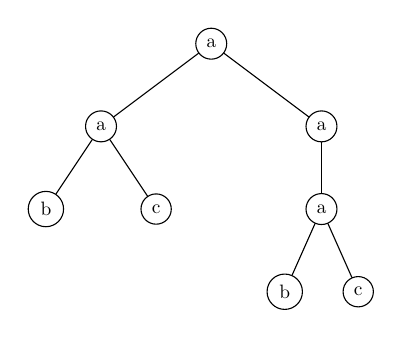
\begin{tikzpicture}[level/.style={sibling distance=40mm/#1}, scale=0.7,transform shape]
\node [circle,draw] (a) {a}
    child {node [circle,draw] (b) {a}
      child {node [circle, draw] {b}}
      child {node  [circle, draw] {c}}
    }
    child {node [circle,draw] (c) {a}
      child {node [circle,draw] (d) {a}
        child {node [circle, draw] {b}}
        child {node [circle, draw] {c}}
      }
    %  child {node [circle, draw] {a}
    %         child {node [circle,draw] (e) {a}
    %           child {node [circle, draw] {b}}
    %           child {node [circle, draw] {c}}
    %         }
    %        }
    };
\end{tikzpicture}
%\caption{An element of $\La_1$}\label{fig:l1}
%\end{subfigure}
\caption{Illustration for Example~\ref{ex:langs-basic}}\label{fig:ex-lang-basic}% While $\La_1$ and $\La_2$ have disjoint images }
\end{figure}




In Example~\ref{ex:langs-basic}, the recognizing algebra is not just 2-distributive but also divides the wreath product of two finite distributive algebras (the language is therefore in PDL).
However, this is not the case in general:
Finite 2-distributive algebras need not divide a wreath product of two \emph{finite} distributive forest algebras.
We will show this in the example below.
The main result of this paper will imply that a wreath product of \emph{four} finite distributive forest algebras will still be enough in this case.
This proves that all languages recognized by finite 2-distributive forest algebras are definable in PDL.




\begin{example}\label{ex:langs}
Consider the following languages (see Figure~\ref{fig:ex-langs} for illustration):

$\La_1$ is the set of nonempty forests where (1) each maximal path has the form $a^* b$ or $a^* c$, (2) each $b$-node has a $c$-sibling, (3) each $c$-node has a $b$-sibling (see Figure~\ref{fig:l1}).

$\La_2$ is the set of nonempty forests where (1) each maximal path has the form $a^* b$ or $a^+ c$, (2) each $b$-node has an $a$-sibling which has a $c$-child, (3) each $a$-node with a $c$-child has a $b$-sibling (see Figure~\ref{fig:l2}).

$\La^a_3$ is the set of (possibly empty) forests where each tree has the form $c_d(f_1 + f_2)$, where $c_d$ denotes the context consisting of only a node labeled $d$ and a variable below it, with $f_1 \in \La^b_3$, $f_2\in \La_1$.

$\La^b_3$ is the set of (possibly empty) forests where each tree has the form $c_d(f_1+f_2)$, with $f_1 \in \La^a_3$ and $f_2 \in \La_2$.

Set $\La := \La^a_3 + \La^b_3$  (see Figure~\ref{fig:l}).

It can be shown that $\La$ is recognized by a wreath product of two infinite distributive algebras and thus is 2-distributive by Proposition~\ref{prop:2-wreath}.
However, $\La$ is not recognized by any wreath product of two \emph{finite} distributive algebras.
%We'll prove this in Appendix~\ref{sec:proof-ex}, and provide a sketch here:

The proof is based on facts about \emph{separation} by morphisms to distributive algebras:
If $\La$ is a language of forests, $\pi(\La) \subseteq Pow(\Sigma^*)$ is the image of $\La$ under $\pi$, a set of finite pathsets.
First, it is not hard to see that $\pi(\La_1) \cap \pi(\La_2)$ is empty, and thus the language $\pi^{-1}(\pi(\La_1))$ separates these: $\La_1 \subset \pi^{-1}(\pi(\La_1)) \subset (H_\Sigma - \La_2)$.
The syntactic forest algebra of $\pi^{-1}(\pi(\La_1))$ is distributive, but infinite (it crucially needs to count at arbitrary depths).
From this fact, one can derive using Theorem~\ref{prop:2-wreath} that $\La$ is indeed 2-distributive.


However, even though $\La_1$ and $\La_2$ are both regular, no language recognized by a \emph{finite} distributive algebra can separate them.
From this, one can deduce using the Derived Category Theorem~\ref{thm:derived-cat}  that $\La$ is not recognized by the wreath product of any two finite distributive forest algebras. % (see Appendix~\ref{sec:proof-ex}). 
However, it is not hard to show that $\La_1$ and $\La_2$ are both recognized by a wreath product of two finite distributive algebras. Fom this, one can derive that $\La$ is recognized by a wreath product of \emph{three} finite distributive forest algebras.
\end{example}





\begin{figure}
\begin{subfigure}[b]{0.3\textwidth}
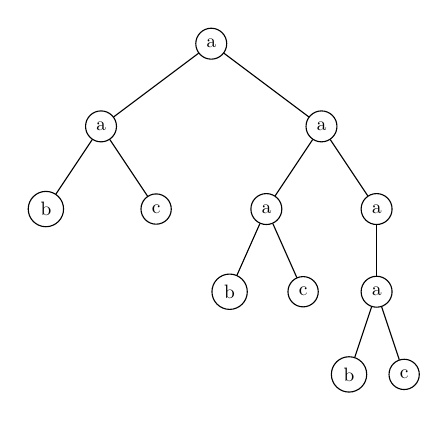
\begin{tikzpicture}[level/.style={sibling distance=40mm/#1}, scale=0.7,transform shape]
\node [circle,draw] (a) {a}
    child {node [circle,draw] (b) {a}
      child {node [circle, draw] {b}}
      child {node  [circle, draw] {c}}
    }
    child {node [circle,draw] (c) {a}
      child {node [circle,draw] (d) {a}
        child {node [circle, draw] {b}}
        child {node [circle, draw] {c}}
      }
      child {node [circle, draw] {a}
             child {node [circle,draw] (e) {a}
               child {node [circle, draw] {b}}
               child {node [circle, draw] {c}}
             }
            }
    };
\end{tikzpicture}
\caption{An element of $\La_1$}\label{fig:l1}
\end{subfigure}
%
%
\begin{subfigure}[b]{0.3\textwidth}
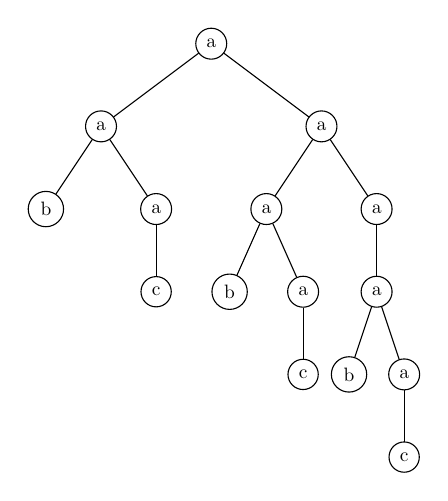
\begin{tikzpicture}[level/.style={sibling distance=40mm/#1}, scale=0.7,transform shape]
\node [circle,draw] (a) {a}
    child {node [circle,draw] (b) {a}
      child {node [circle, draw] {b}}
      child {node  [circle, draw] {a} child {node  [circle, draw] {c}}   }
    }
    child {node [circle,draw] (c) {a}
      child {node [circle,draw] (d) {a}
        child {node [circle, draw] {b}}
        child {node  [circle, draw] {a} child {node  [circle, draw] {c}}   }
      }
      child {node [circle, draw] {a}
             child {node [circle,draw] (e) {a}
               child {node [circle, draw] {b}}
               child {node  [circle, draw] {a} child {node  [circle, draw] {c}}   }
             }
            }
    };
\end{tikzpicture}
\caption{An element of $\La_2$}\label{fig:l2}
\end{subfigure}
%
%
%
\begin{subfigure}[b]{0.3\textwidth}
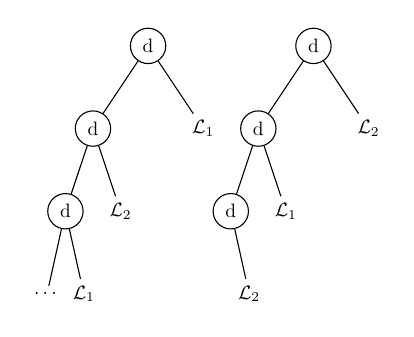
\begin{tikzpicture}[level/.style={sibling distance=20mm/#1}, scale=0.7,transform shape]
\node at (0,0) [circle,draw] (1st) {d}
    child {node [circle,draw] (b) {d}
      child {node [circle, draw] {d}
        child {node  {$\dots$}} % edge from parent[draw=none]}
        child {node  {$\La_1$}}
       }
      child {node   {$\La_2$}}
    }
    child {node  {$\La_1$}};
\node at (3,0) [circle,draw] (a) {d}
    child {node [circle,draw] (b) {d}
      child {node [circle, draw] {d}
        child {node  {} edge from parent[draw=none]}
        child {node {$\La_2$}}            }
      child {node   {$\La_1$}}
    }
    child {node   {$\La_2$}};
\end{tikzpicture}
\caption{A schematic depiction of $\La$: The left tree belongs to $\La_3^a$, the right tree one to $\La_3^b$.}\label{fig:l}
\end{subfigure}
\caption{Illustration for Example~\ref{ex:langs}. $\La$ is 2-distributive and regular, but not recognized by the wreath product of two finite distributive forest algebras.}\label{fig:ex-langs}% While $\La_1$ and $\La_2$ have disjoint images }
\end{figure}


%\subsection{k-Distributivity}

%\emph{Not sure whether to put this definition in the paper, and if yes where to put it.}
\section{The Derived Forest Category}\label{sec:categories}


The proof of our main result will construct wreath product decompositions by separately studying the left and right factors of a wreath product.
Given a 2-distributive forest algebra $(H_2, V_2)$, we will use the Separation Lemma~\ref{cor:separation} to construct an intended right-hand factor $(H_2, V_2)$ which is already known to be a wreath product of finite distributive forest algebras.
The remaining problem is then to find a left-hand factor $(H,V)$ such that
%
%
%To obtain the right factor of a wreath product decomposition, we prove a separation result.
%To then obtain the left factor, we start at the Derived Category, and show that it has a certain local property -- in our case, local distributivity.
%To conclude a decomposition result, we then prove that this local property entails a global property of the 
%
%These steps are remarkably similar to results from the theory of logic on words and finite monoids which also reduce the problem of decidability to separation \cite{place-going-2014} and local-global theorems \cite{krebs-effective-2012}.
%
%
%
%We will be in the setting where we have surjective forest algebra morphisms
%$$(H_1, V_1) \xleftarrow{\alpha} \Sigma^\Delta \xrightarrow{\beta} (H_2, V_2)$$
%We will want to give a wreath product `decomposition' of $(H_1,V_1)$ into some product $(H,V) \wr (H_2,V_2)$ -- that is, we want to decompose an algebra when the right-hand side is given.
%More formally, we seek conditions on forest algebras $(H,V)$ under which
\begin{equation}\label{eq:wreath-eq}
(H_1,V_1) \prec (H,V) \wr (H_2,V_2)
\end{equation}
holds. If we can show that this factor can be chosen to be distributive, the problem is solved.
In order to do this, we seek a general strategy to obtain a `minimal' left-hand factor $(H,V)$.
%While it is not hard to find such algebras (e.g., $(H_1,V_1)$ will do), we seek an `optimal' solution $(H,V)$.
%
In the case of groups, the solution to this problem is provided by the kernel group, $\operatorname{ker}\ \phi$, when $\phi : G\rightarrow H$: Then $G$ is embedded in $\operatorname{ker} \phi \wr H$.

For monoids, the analog to $\operatorname{ker} \phi$ is not a monoid any more, but a category.
This classical construction is known as the \emph{Derived Category}~(\cite{tilson-categories-1987}, \cite{rhodes-q-theory-2009}) and originated from the study of regular word languages via wreath products of finite monoids \cite{brzozowski-characterizations-1973}, \cite{therien-graph-1985}, \cite{straubing-finite-1985}.
Recently, \cite{straubing-forest-2018} showed that this construction generalizes to the setting of forest algebras.

The sense in which this construction is `optimal' is made precise in Tilson's Derived Category Theorem~\cite{tilson-categories-1987}.
In the case of forest algebras, we will essentially see that the decomposition in (\ref{eq:wreath-eq})
holds if and only if $(H,V)$ is divided by a certain forest category determined from $(H_1,V_1)$ and $(H_2,V_2)$ and morphisms from $\Sigma^\Delta$ into these, where the notion of `division' by a category will be made precise below.

In this section, we will review the definition of the Derived Forest Category and the Derived Category Theorem from \cite{straubing-forest-2018}.
The Derived Forest Category is a category with some structure added to it, and the relation between forest categories and categories is akin to the relation between forest algebras and monoids.
It is possible to define a general notion of Forest Categories \cite{straubing-forest-2018}, but for our purposes, it is sufficient to consider the Derived Forest Category:

%In this setting, there are often two parts to proving a wreath decomposition for an algebra:
%First to establish a property of the derived category, and then verifying that this property implies division of an algebra of a desired kind.
%The Derived Category Theorem then allows to conclude that the algebra indeed 
%This will indeed be the proof strategy of our main result:
%We will show that a certain derived category satisfies a local version of distributivity, and then 


%In the classical setting of finite monoids, a fruitful tool for studying the wreath product is Tilson's theory of finite categories.
%
%It provides a general tool for `decomposing' a monoid into a wreath product with a given right-hand factor.
%In the case of groups, when $\phi : G\rightarrow H$ is a group morphism, then $G$ is embedded in the wreath product $ker \phi \wr H$.
%In the case of general monoids, such a construction is not possible in general.
%It is of course, given $M_1, M_2$, possible to find a monoid $M_3$ such that $M_1 \prec M_3 \wr M_2$.
%However, in order to find a `minimal' or `optimal' such $M_3$, it becomes necessary to generalize 
%
%
%The basic idea is that, given two monoids $M_1, M_2$, the derived category construction provides a `minimal' $C$ such that $M_1 \prec C \wr M_2$.
%
%
%
%Unlike finite groups, in the case of finite monoids, this `minimal' object is not a monoid in general, but a category.
%The construction TODO
%A basic tool will be a generalization of the classical theory of derived categories to the setting of forest algebras introduced by \cite{straubing-forest-2018}:

\begin{defin}\label{def:derived-category}[Derived Forest Category, \cite{straubing-forest-2018}]
Let $\Sigma$ be a finite alphabet. Consider a pair of surjective forest algebra morphisms
$$(H_1, V_1) \xleftarrow{\alpha} \Sigma^\Delta \xrightarrow{\beta} (H_2, V_2)$$
The derived category $D_{\alpha,\beta}$ is defined as follows:
\begin{enumerate}
\item The set of \emph{objects} of the category is $\Obj(D_{\alpha,\beta}) := H_2$
\item As in ordinary categories, \emph{arrows} connect objects.
To define the arrows, we fix $h, h' \in H_2$ and introduce an equivalence relation on the set of triples $(h,p,h')$ with $p \in V_\Sigma$ for which $\beta(p)\cdot h=h'$. We set $(h,p,h')\sim(h,q,h')$ if for all $s\in H_ \Sigma$ with $\beta(s)=h$, we have $\alpha(ps) = \alpha(qs)$.

We then set $\Arr(h,h')$ to be the set of equivalence classes of $\sim$.
Its elements are called \emph{arrows}.

We depict an arrow as $\carrow{h}{p}{h'}$, with the understanding that the same arrow can have many distrinct representations in this form.

For consistency with notation here, the direction of arrows in this graphical notation is inverted relative to \cite{straubing-forest-2018}.

%(Note: I've inverted the direction of arrows compared to Howard's writeup to make it compatible with the order of $V$ and $H$ elements in this document).

\item To obtain a category, we now want to define the multiplication of arrows. We set
$$\left( \carrow{h_2}{p}{h_3}\right)\cdot\left(\carrow{h_1}{q}{h_2}\right)=\carrow{h_1}{pq}{h_3}$$
or shortened
$$\carrow{\carrow{h_1}{q}{h_2}}{p}{h_3}=\carrow{h_1}{pq}{h_3}$$
%Observe that $h_1\beta(pq) = h_1\beta(p)\beta(q) = h_2\beta(q)=h_3$, so the right-hand side of the above equation is indeed the representation of an arrow.
It can be shown that this is a well-defined arrow, independently of the representation chosen for the arrows \cite{straubing-forest-2018}.
Since the multiplication on $V_\Sigma$ is associative, this multiplication is associative.
The arrow $\carrow{h}{1_{V_\Sigma}}{h}$ is the identity at $h\in H_2$.

%We still need to show that this is well-defined; in other words, that
%$$(h_1,p,h_2)\sim(h_1,p',h2),(h_2,q,h_3)\sim(h_2,q,h_3)$$
%implies
%$$(h_1,pq,h_3)\sim(h_1,p'q',h_3)$$
%To this end, let $s\in H_\Sigma$ and $\beta(s)=h_1$. Then the two equivalences imply $$\alpha(sp)=\alpha(sp')$$ and, since $\beta(sp)=h_2$, $$\alpha(spq)=\alpha(spq')$$ so the two together give $$\alpha(spq)\alpha(sp'q')$$ as required.
%Associativity follows at once from associativity in $V_\Sigma$, and the arrow $h\xrightarrow{1_{V_\Sigma}}h$ is the identity at $h\in H_2$.

Up to this point, we have defined a category. We now add some additional structure:

\item For $h \in H_2$, we set
$$\HArr(h) := \{(\alpha(s), h) : s \in H_\Sigma, \beta(s) = h\}$$
The elements of this set are called \emph{half-arrows}. They can be thought of as being arrows that end in an object, but do not start in any object.
%While arrows are analogous to context types in forest algebras, half-arrows are analogous to forest types.

We depict the half-arrow $(h_1, h_2)$ as $\carrow{}{h_1}{h_2}$.

\item We set $\HArr(D_{\alpha,\beta})$ to be the set of all half-arrows. Note that $\Obj(D_{\alpha,\beta})$ and $\HArr(D_{\alpha,\beta})$ are monoids, and that the projection of a half-arrow onto the second element (that is, the object at the end of the arrow in our graphical notation) is a homomorphism from $\HArr(D_{\alpha,\beta})$ to $\Obj(D_{\alpha,\beta})$.%, as required in the definition.
%We must now define the other operations in the category and show that they have the desired properties. We set


\item Viewed in analogy to forest algebras, arrows correspond to context types, while half-arrows correspond to forest types. We therefore want arrows to act on half-arrows. We define the action of an arrow on a half-arrow by
$$\left(\carrow{h_2}{p}{h_2'}\right)\cdot\left(\carrow{}{h_1}{h_2}\right)=\carrow{}{\alpha(p)h_1}{h_2'}$$
or shortened
$$\carrow{\carrow{}{h_1}{h_2}}{p}{h_2'}=\carrow{}{\alpha(p)h_1}{h_2'}$$
%(proof of well-definedness in \cite{straubing-forest-2018})
\item In analogy to forest algebras, we want to be able to add arrows and half-arrows. We set
$$\left(\carrow{h}{p}{h'}\right)+\left(\carrow{}{h_1}{h_2}\right) = \carrow{h}{p+s}{\left(h'+h_2\right)}$$
where $s\in H_\Sigma$ such that $\alpha(s) = h_1$, $\beta(s)=h_2$.
%(correctness proof in \cite{straubing-forest-2018})
\end{enumerate}
For proofs of well-definedness, we refer the reader to  \cite{straubing-forest-2018}.
\end{defin}

%It is possible to define a general notion of forest categories, but for our purposes, it is enough to reason about derived categories.
%It can be shown that $D_{\alpha, \beta}$ is a forest category in the general sense defined in the appendix.
%For our purposes, it is enough to reason about derived categories.
%In the rest of this paper, when we say `category', we can assume that it is actually equal to some $D_{\alpha,\beta}$.
%All forest categories here will be finite, that is, the sets of objects, arrows, and half-arrows will all be finite.


To formulate the Derived Category Theorem connecting Derived Categories with wreath products, it is necessary to generalize the notion of division to the setting of forest categories dividing forest algebras:

\begin{defin}\label{def:division}[Division, \cite{straubing-forest-2018}]
If $C$ is a derived forest category and $(H,V)$ a forest algebra, then we write $C\prec(H,V)$, and say $C$ \emph{divides} $(H,V)$, if for each $\left(\carrow{}{c}{x}\right) \in \HArr(C)$ there exists a nonempty set $K_{\carrow{}{c}x} \subseteq H$, and for each $\left(\carrow{x}{d}{y}\right)\in \Arr(C)$ there exists a nonempty set $K_{\carrow{x}{d}{y}}\subseteq V$ satisfying the following properties:
\begin{enumerate}
\item (Preservation of Operations) For all $\carrow{}{c}x$, $\carrow{}{d}y \in \HArr(C)$, $\carrow{x}{e}{y}, \carrow{y}{f}{z} \in \Arr(C)$,
\begin{enumerate}
\item $K_{\carrow{y}{f}{z}} \cdot K_{\carrow{x}{e}{y}} \subseteq K_{\carrow{\carrow{x}{e}{y}}{f}{z}}$
\item $K_{\carrow{x}{e}y} \cdot K_{\carrow{}{c} x} \subseteq K_{\carrow{\carrow{}{c}{x}}{e}{y}}$
\item $K_{\carrow{}{c}x}+K_{\carrow{}{d}y}\subseteq K_{\carrow{}{c}{x}+\carrow{}{d}{y}}$
\item $K_{\carrow{}{c}x} + K_{\carrow{y}{f}z} \subseteq K_{\carrow{}{c}x+y\carrow{}{f}z}$
\item $K_{\carrow{y}{f}z} + K_{\carrow{}{c}x} \subseteq K_{\carrow{y}{f}z+\carrow{}{c}x}$
\end{enumerate}
\item (Injectivity)
\begin{enumerate}
\item If $\carrow{x}{c}y$ and $\carrow{x}{c'}y$ are distinct arrows, then $K_{\carrow{x}{c}y}\cap K_{\carrow{x}{c'}y} = \emptyset$
\item If $\carrow{}{c}y$ and $\carrow{}{c'}y$ are distinct half-arrows, then $K_{\carrow{}{c}y}\cap K_{\carrow{}{c'}y}=\emptyset$.
\end{enumerate}
\end{enumerate}

\end{defin}

In the special case where a derived forest category has exactly one object, it can be viewed as a forest algebra.
In this case, the notion of division reduces to ordinary division of forest algebras.

We are now ready to state the Derived Category Theorem connecting categories with wreath products.
We state only the direction required for our main result:

\begin{theorem}\label{thm:derived-cat}[Derived Category Theorem,  \cite{straubing-forest-2018}]
Let $\Sigma$ be an alphabet, and let $\alpha, \beta$ be morphisms from $\Sigma^\Delta$ onto forest algebras $(H_1, V_1)$, $(H_2, V_2)$, respectively. Let $(H,V)$ be a forest algebra.
Assume $D_{\alpha, \beta} \prec (H,V)$. Then
$$(H_1,V_1) \prec (H,V) \wr (H_2, V_2)$$
\end{theorem}

%The converse is stated as Theorem~\ref{thm:full:deriv} in the Appendix, but is not required for our main result.


\section{Main Result}\label{sec:main-result}

Our aim is to prove that any language recognized by a finite 2-distributive forest algebras is definable in PDL: 


\begin{theorem}\label{thm:main-result}
Let $\Ff$ be a finite 2-distributive forest algebra.
Then every language recognized by $\Ff$ is definable in PDL.
\end{theorem}
In the Discussion (Section~\ref{sec:discussion}), we will discuss the relevance of this result for the question of deciding definability in PDL.

Our proof proceeds by solving two sub-problems related to the left and right factors in wreath product decompositions:
To obtain the right factor of a wreath product decomposition, we study the problem of \emph{separating} forest languages by the map $\pi$.
To then obtain the left factor, we start at the Derived Category, and show that it has a certain local property -- in our case, local distributivity.
To conclude a decomposition result, we then prove that this local property entails a global property.
These steps are remarkably similar to results from the theory of logic on words and finite monoids which also reduce the problem of decidability to separation \cite{place-going-2014} and Local-Global theorems \cite{krebs-effective-2012}.



%Notation: $DISTR \wr DISTR$ is the Birkhoff variety of forest algebras generated by wreath products $X \wr Y$ ($X,Y \in DISTR$).




\subsection{Separation Lemma}
We will first state the Separation Lemma.
Recall that $\pi(f)$ is the set of paths in the forest $f$.
If $\La$ is a language of forests, $\pi(\La) \subseteq Pow(\Sigma^*)$ is the image of $\La$ under $\pi$, a set of finite pathsets.

\begin{llemma}[Separation Lemma]\label{cor:separation}
Let $\La_1, \La_2 \subseteq H_\Sigma$ be regular forest languages such that
$$\pi(\La_1) \cap \pi(\La_2) = \emptyset$$
Then there are finite distributive algebras $\Ff_1, \Ff_2, \Ff_3$ and a language $X \subseteq \Sigma^\Delta$ recognized by $\Ff_1\wr\Ff_2\wr\Ff_3$ such that $$\La_1 \subseteq X \subseteq (H_\Sigma - \La_2)$$
That is, $X$ \emph{separates} $\La_1$ from $\La_2$.
\end{llemma}

\begin{proof}
%This is shown in Appendix~\ref{sec:sep}, using a combinatorial result shown in Appendix~\ref{sec:main-lemma}.
The proof considers a forest algebra $(H,V)$ recognizing both $\La_1$ and $\La_2$ via a morphism $\phi$, and constructs PDL languages `approximating' each $\phi^{-1}(h)$ for $h \in H$.
\end{proof}

Let's consider how this is useful for proving Theorem~\ref{thm:main-result} by sketching the proof idea for the theorem -- we will make this more precise in Section~\ref{rect:result-proof}.
If $\Ff$ is a forest algebra with morphism $\phi_\Ff : \Sigma^\Delta \rightarrow \Ff$, we can apply this lemma to all pairs of languages $\phi_\Ff^{-1}(h)$ for $h \in H_\Ff$ and obtain separators $X_{h,h'}$ for each pair whenever $\pi\phi^{-1}(h)\cap\pi\phi^{-1}(h') = \emptyset$.
Combining the resulting separators, we can build finite distributive algebras $\Ff_1, \Ff_2, \Ff_3$ and a morphism $\phi_X : \Sigma^\Delta \rightarrow \Ff_1\wr\Ff_2\wr\Ff_3$ which recognizes each $X_{h,h'}$.
We will examine the derived category $D_{\phi_\Ff, \phi_X}$.
If we can show that this derived category divides a finite distributive algebra $\Ff_0$, we can apply the Derived Category Theorem to conclude $\Ff \prec \Ff_0 \wr \Ff_1 \wr \Ff_2 \wr \Ff_3$, which then will prove Theorem~\ref{thm:main-result}.

\subsection{Locally-Distributive Categories}
Recall the equation $v [h_1 + h_2] = v h_1 + v h_2$ defining distributive forest algebras.
To apply this to derived forest categories, we would want to interpret $v$ as an arrow and $h_1, h_2$ as half-arrows.
In general, this equation does not make sense, since the action of an arrow on a half-arrow is only defined in certain cases. %an arrow can only act on certain half-arrows.
The equation becomes sensible when we restrict it to those arrows and half-arrows for which the action is defined:

\begin{defin}[Locally Distributive]\label{def:loc-dist}
We say that a derived forest category $C$ is \emph{locally distributive} if the following equation holds
for any $h \in \Obj(C)$ and any two half-arrows $h_1, h_2 \in \HArr(h)$, and for any arrow $v \in \Arr(h,h')$ ($h' \in \Obj(C)$):
$$v [h_1 + h_2] = v h_1 + v h_2$$
Rewriting this in arrow-based notation, we want the following for any half-arrows $\carrow{}{h_1}h$ and $\carrow{}{h_2}h$, and for any arrow $\carrow{h}{v}{h'}$:
$$\left(\carrow{h}{v}{h'}\right)\cdot\left(\carrow{}{h_1}h + \carrow{}{h_2}h\right) = \left(\carrow{\carrow{}{h_1}{h}}{v}{h'}\right) + \left(\carrow{\carrow{}{h_2}{h}}{v}{h'}\right)$$
\end{defin}

Any derived forest category that divides a distributive forest algebra must be locally distributive.
We now show that the converse is also true: Any locally-distributive category divides some distributive forest algebra.
In analogy to results from the theory of ordinary finite categories, we refer to this as a Local-Global Theorem -- showing that being locally distributive entails a global property of the category:

\begin{theorem}[Local-Global]\label{thm:loc-glob}
Let $C$ be a locally-distributive finite derived forest category.
Then it divides a finite distributive forest algebra.
\end{theorem}



\begin{proof}
%See Appendix~\ref{sec:locglob}.
The proof proceeds by considering terms built from arrows and half-arrows and using local distributivity to transform them into a normal form that only depends on the paths in these terms (viewing them as forests). %, made precise in Appendix \ref{sec:locglob}).
We then apply Proposition~\ref{prop:distr-char} to construct a finite distributive forest algebra and a division.
\end{proof}







The idea of introducing a `local' version of distributivity that is appropriate for forest categories, and then relating it to distributive forest algebras in a `Local-Global' Theorem is related to a long tradition in the theory of semigroups and monoids, where local pseudovarieties of categories have been an important object of study (e.g., \cite{tilson-categories-1987}, \cite{pin-locally-1988}, \cite{almeida-syntactical-1996}), and where such Local-Global theorems have been applied to prove decidability of logic classes~\cite{krebs-effective-2012}.

In order to prove Theorem~\ref{thm:main-result}, our goal will be to prove that the derived category $D_{\phi_\Ff, \phi_X}$ mentioned above is locally distributive, then being able to apply Theorem~\ref{thm:loc-glob}.
The details are given in Section \ref{rect:result-proof}.




%\begin{figure*}
%\begin{subfigure}[b]{0.3\textwidth}
%\begin{center}
%\begin{tikzpicture}[level/.style={sibling distance=40mm/#1}, scale=0.7,transform shape]
%\node [circle,draw] (a) {$h \xleftarrow{v} \left(h' + h''\right)$}
%    child {node [circle,draw] (b) {$h' \xleftarrow{h_1}$}
%    }
%    child {node [circle,draw] (c) {$h'' \xleftarrow{h_2}$}
%    };
%\end{tikzpicture}
%\end{center}
%\caption{}\label{fig:diag-basic}
%\end{subfigure}
%%
%\begin{subfigure}[b]{0.3\textwidth}
%\begin{center}
%\begin{tikzpicture}[level/.style={sibling distance=40mm/#1}, scale=0.7,transform shape]
%\begin{scope}[xshift=-1cm]
%\node [circle,draw] (a) {$h' \xleftarrow{v} h$}
%    child {node [circle,draw] (b) {$h \xleftarrow{h_1}$}
%    };
%\end{scope}
%\begin{scope}[xshift=1cm]
%\node [circle,draw] (c) {$h' \xleftarrow{v} h$}
%    child {node [circle,draw] (d) {$h \xleftarrow{h_2}$}
%    };
%\end{scope}
%\end{tikzpicture}
%\end{center}
%\caption{}\label{fig:diag-sep}
%\end{subfigure}
%%
%\begin{subfigure}[b]{0.3\textwidth}
%\begin{center}
%\begin{tikzpicture}[level/.style={sibling distance=40mm/#1}, scale=0.7,transform shape]
%\node [circle,draw] (a) {$h' \xleftarrow{v} h$}
%    child {node [circle,draw] (b) {$h \xleftarrow{h_1}$}
%    }
%    child {node [circle,draw] (c) {$h \xleftarrow{h_2}$} };
%\end{tikzpicture}
%\end{center}
%\caption{}\label{fig:diag-together}
%\end{subfigure}
%%
%%
%%
%\caption{Examples of forest diagrams. In any locally distributive derived forest category, the diagrams in (b) and (c) result in the same value under the map $\operatorname{Val}$.}\label{fig:diagrams}% While $\La_1$ and $\La_2$ have disjoint images }
%\end{figure*}





%\begin{proof}[Proof Sketch for the Local-Global Theorem~\ref{thm:loc-glob}]
%Let $C$ be a finite and locally-distributive derived forest category.
%To prove the Local-Global Theorem, we will need the notion of \emph{forest diagrams}:
%
%A \emph{forest diagram} is a forest whose leaves are labeled with half-arrows of $C$ and whose internal nodes are labeled with arrows of $C$, subject to the following consistency condition: Let $n$ be a (non-leaf) node labeled with an arrow $\carrow{h_1}{v}{h_2}$, and let $h_3, ..., h_k \in \Obj(C)$ be the endpoints of the arrows or half-arrows that label the root nodes of the children of $n$. Then $h_3 + ... + h_k = h_1$.
%Examples are shown in Figure~\ref{fig:diagrams}.
%
%To any forest diagram one can assign a half-arrow of $C$ by recursively adding up the half-arrows assigned to siblings, and multiplying out the action of arrows on the half-arrows assigned to their children.
%Let $\operatorname{Val}$ be the map assigning these values to forest-diagrams.
%Each forest-diagram is a forest in $H_{\Sigma_C}$, where $\Sigma_C$ consists of the arrows and half-arrows of $C$.
%From the definition of locally-distributive, one can show that, for forest diagrams $d$, $\operatorname{Val}(d)$ is determined by $\pi(d)$. 
%That is, for distinct half-arrows $\carrow{}{c}h$, $\carrow{}{c'}{h'}$,
%$$\pi(\operatorname{Val}^{-1}(\carrow{}{c}h)) \cap \pi(\operatorname{Val}^{-1}(\carrow{}{c'}{h'})) = \emptyset$$
%
%Certainly, the sum of the two half-arrows has to be distinct from at least one of them:
%At least, $\carrow{}{c}h + \carrow{}{c'}{h'} \neq \carrow{}{c}h$ or $\carrow{}{c}h + \carrow{}{c'}{h'} \neq \carrow{}{c'}{h'}$.
%We'll assume that the first one holds.
%Then, we know
%$\pi(\operatorname{Val}^{-1}(\carrow{}{c}h + \carrow{}{c'}{h'})) \cap \pi(\operatorname{Val}^{-1}(\carrow{}{c}h)) = \emptyset$
%For any forest language $\La$, we define $\Pi(\La)\subseteq (\Sigma_C)^*$ to be %the set of all paths occurring in some forest in $\La$:
%$\Pi(\La) := \bigcup_{f \in \La} \pi(f)$
%
%Now consider the sets
%$\Pi_1 := \Pi(\operatorname{Val}^{-1}(\carrow{}{c}h))$ and 
%$\Pi_2 := \Pi(\operatorname{Val}^{-1}(\carrow{}{c'}{h'}))$.
%One can show that, in order to separate forest diagrams evaluating to $\carrow{}{c}h$ from those evaluating to $\carrow{}{c'}{h'}$, it is sufficient to check whether the pathset of the diagram in question contains an element of $\Pi_1-\Pi_2$.
%Furthermore, one can show that $\Pi_1, \Pi_2 \subset \Sigma_C^*$ are regular word languages.
%Thus, by Proposition~\ref{prop:distr-char}, some finite distributive forest algebra $\Ff$ recognizes the set of forests whose path set intersects $\Pi_1-\Pi_2$.
%Repeating this argument for all pairs of distinct half-arrows and letting $\widehat{\Ff}$ be the direct product of the obtained distributive algebras, we can construct a division $C \prec \widehat{\Ff}$.
%\end{proof}
%






%\subsection{Proof Sketch for Separation Lemma}
%
%In this section, we provide a coarse sketch of the proof of the separation lemma.
%
%\begin{defin}\label{def:pathsets}[Pathsets: $\pi$, $\freedisth$, $\Pi$]
%Recall the map $\pi : H_\Sigma \rightarrow Pow(\Sigma^*)$ mapping forests to their path sets.
%The image of $\pi$ is called $\freedisth$. That is, $\freedisth$ is the set of nonempty finite subsets of $\Sigma^*$ that are closed under prefixes ($wv \in X \Rightarrow w \in X$).
%%Thus, $\freedisth \subseteq Pow(\Sigma^*)$.
%
%We extend $\pi$ to an operation on forest languages:
%\[\pi(\La) := \{\pi(f) : f \in \La\} \subset Pow(\Sigma^*)\] for $\La \subseteq H_\Sigma$.
%
%When $\La \subseteq H_\Sigma$, then $\Pi(\La)\subseteq \Sigma^*$ is the set of all paths occurring in some forest in $\La$:
%$$\Pi(\La) := \bigcup_{f \in \La} \pi(f)$$
%
%Since $\Pi$ is defined in terms of $\pi$, $\Pi$ is also well-defined on subsets of $\freedisth$: If $X \subseteq \freedisth$, then $\Pi(X) := \bigcup_{\phi \in X} \phi$.
%\end{defin}
%
%\begin{prop}\label{prop:pi-reg}
%Let $\La \subset H_\Sigma$ be a regular forest language. Then $\Pi(\La) \subset \Sigma^*$ is a regular word language, and can be effectively constructed from (an automaton for) $\La$.
%\end{prop}
%
%We are given regular forest languages $\La_1, \La_2$. We want to show that, if the images of $\La_1, \La_2$ under $\pi$ are disjoint, then some language recognized by a wreath product of three finite distributive algebras separates $\La_1, \La_2$.
%
%We will prove a stronger statement to `load the induction hypothesis'.
%This stronger statement will be the Main Lemma~\ref{prop:main-lemma}.
%In order to state and prove it, a few more notions are needed.
%
%We will need a notion of \emph{rules} that is analogous to transitions in bottom-up tree automata:
%
%\begin{defin}[Rules]\label{def:algebras}\label{d:p:ls-lr}
%Let $\Ff = (H,V)$ be a forest algebra, and $\phi : \Sigma^\Delta \rightarrow (H,V)$ a morphism.
%
%A \emph{rule} is a tuple $$(h_0, \alpha, \{h_1, ..., h_k\}) \in H \times \Sigma \times Pow(H)$$ such that $$h_0 = \phi(\alpha)[h_1 + ... + h_k]$$
%The set of rules for $\Ff = (H,V)$ with morphism $\phi$ is called $Rules(\Ff, \phi)$.
%
% For $\rho \in Rules(\Ff)$, let $\La(\rho)$ be the set of nonempty forests where all top-level rule applications are of rule $\rho = (h_0, \alpha, \{h_1, ..., h_k\})$.
%Formally, a nonempty forest $f$ belongs to $\La(\rho)$ iff, for any tree $t \in f$, (1) the root symbol of $t$ is $\alpha$, and (2) if $C$ is the set of trees that are children of the root node of $t$, then $\{\phi(c) :c \in C\} = \{h_1, ... , h_k\}$.
%
%For convenience, we will use the same notation for elements of $H$: $\La(h) := \phi^{-1}(h)$ for $h \in H$.
%\end{defin}
%
%
%\begin{llemma}[Main Lemma]\label{prop:main-lemma}
%Let $\Ff = (H,V)$ be a finite forest algebra, and $\phi : \Sigma^\Delta\rightarrow(H,V)$ a morphism.
%There is a map $\Pa$ assigning to each $\rho \in Rules(\Ff)$ a language $\Pa(\rho) \subseteq H_\Sigma$ such that the following four statements hold: %recognized by a wreath product of two finite distributive algebras, such that the following holds:
%
%(A) For any $\rho \in Rules(\Ff,\phi)$, we have $$\La(\rho) \subseteq \Pa(\rho)$$
%
%
%(B) For all $\rho, \rho' \in Rules(\Ff,\phi)$,
%$\Pa(\rho) \cap \Pa(\rho')$ is empty if and only if $\pi\La(\rho) \cap \pi\La(\rho')$ is empty.
%%and for all $n \in \N$:
%%$$\Pi \Rn (\Pa(\rho) \cap \Pa(\rho')) = \Pi\Rn(\pi\La(\rho) \cap \pi\La(\rho'))$$
%
%(C) For any $\rho_1, ... \rho_k \in Rules(\Ff,\phi)$, the language $$\{f = f_1 + ... + f_k : f_i \in \Pa(\rho_i)\}$$
%is recognized by a wreath product of three finite distributive forest algebras.
%
%(D) For any $\rho \in Rules(\Ff,\phi)$ and any forest $f = \{t_1, ..., t_l\}$, where each $t_i$ is a tree, we have $f \in \Pa(\rho)$ if and only if all the  singleton forests $\{t_i\}$ ($i = 1, ..., l$) are in $\Pa(\rho)$.
%%$\{t_1, ..., t_l\}$, 
%\end{llemma}
%
%
%%For the proof of the Main Lemma, we will utilize the following bit of notation.
%%Recall the set $\freedisth$ from Definition~\ref{def:pathsets}.
%%\begin{defin}
%%Let $\Ff = (H,V)$.
%%Let $R, S \subseteq Rules(\Ff,\phi)$ or $R, S \subseteq H$.
%%Then $\left\langle R, S\right\rangle$ is a subset of $\freedisth$ defined as follows:
%%
%%$d \in \left\langle R, S\right\rangle$ if and only if there are forests $f_1, f_2$ such that $\pi(f_1) = \pi(f_2) = d$, and there are 
%%$r_1, ..., r_n \in R$, $s_1, ..., s_k \in S$ ($n, k > 0$) and
%%$$f_1 \in \La(r_1) + ... + \La(r_n)$$
%%$$f_2 \in \La(s_1) + ... + \La(s_k)$$
%%\end{defin}
%%Recall the operation $\Pi$ mapping forest languages to subsets of $\Sigma^*$.
%%We will also apply it to subsets of $\freedisth$: For $X \subseteq \freedisth$, set $\Pi(X) := \bigcup_{x \in X} x$.
%%
%%
%%\begin{defin}\label{def:height}
%%The \emph{height} of a forest is the length of the longest paths. Formally, we define $\height(\alpha[C]) := 1 + \max_{t \in C} \height(t)$, with $\max \emptyset := 0$.
%%If $f$ is a forest, we set $\height(f) := \max_{t \in f} \height(t)$, with $\max\emptyset := 0$.
%%
%%We will frequently use:
%%$$Z_n(\La) := \{f \in \La: \height f \leq n\}$$% forests in $\La$ of depth $\leq n$% (was called $R^n$ in the previous writeup)
%%
%%Since the height of a forest only depends on its pathset and the elements of $\freedisth$ are finite sets, we can write $Z_n X$ even when $X \subseteq \freedisth$.
%%
%%%\end{enumerate}
%%\end{defin}
%%
%%
%%
%%\begin{llemma}[Stronger Version of Main Lemma]\label{prop:main-lemma-strong}
%%Let $\Ff = (H,V)$ be a finite forest algebra, and $\phi : \Sigma^\Delta\rightarrow(H,V)$ a morphism.
%%There is a map $\Pa$ assigning to each $R \subseteq Rules(\Ff)$ a language $\Pa(R) \subseteq H_\Sigma$ such that the following four statements hold: 
%%
%%(A) For any $R \subseteq Rules(\Ff,\phi)$, and for any $\rho_1, ..., \rho_k \in R$ ($r \geq 1$), we have $$\La(\rho_1) + ... + \La(\rho_k) \subseteq \Pa(R)$$
%%
%%That is, $\Pa(R)$ extends the languages obtained by adding forests that evaluate to rules in $R$.
%%
%%(B) The following relationship between $\Pa(\cdot)$ and the construct $\left\langle\cdot,\cdot\right\rangle$ holds
%%for all $R, S \subseteq Rules(\Ff,\phi)$, and $n \in \N$: 
%%$$\Pi \left(\Rn\Pa(R) \cap \Rn\Pa(S)\right) =  \Pi \Rn \left\langle R, S \right\rangle$$
%%In words: The following two operations yield the same sets of paths:
%%
%%\begin{enumerate}
%%\item Intersect the languages $\Pa(R)$, $\Pa(S)$, restricted to forests of height $\leq n$. Then compute the set of paths occurring in the resulting forest language. 
%%\item Compute the set $\left\langle R, S\right\rangle \subseteq \freedisth$, and restrict to pathsets of height $\leq n$. Then compute the set of paths, that is, the union over the resulting subset of $\freedisth$.
%%\end{enumerate}
%%
%%(C) For any $\rho_1, ... \rho_k \in Rules(\Ff,\phi)$, the language $$\{f = f_1 + ... + f_k : f_i \in \Pa(\{\rho_i\})\}$$
%%is recognized by a wreath product of three finite distributive forest algebras.
%%
%%(D) For any $R \subseteq Rules(\Ff,\phi)$ and any forest $f = \{t_1, ..., t_l\}$ (each $t_i$ being a tree), we have $f \in \Pa(R)$ if and only if all the singleton forests $\{t_i\}$ ($i = 1, ..., l$) are in $\Pa(R)$.
%%\end{llemma}
%%
%%
%%
%%Each $\Pa(\rho)$ can be seen as a PDL approximator of the language $\La(\rho)$.
%%While (A) guarantees that these approximators are sufficiently `large', (B) guarantees that they suffice to construct a PDL separator whenever $\La(\rho)$ and $\La(\rho')$ are separable by $\pi$ at all.
%%We'll prove the Main Lemma below in Appendix~\ref{sec:main-lemma}. Using the Main Lemma, we prove the Separation Lemma:
%%
%%\begin{proof}[Proof of the Separation Lemma~\ref{cor:separation}]
%%Since $\La_1, \La_2$ are regular, there is a finite forest algebra $\Ff = (H,V)$ which recognizes both $\La_1$ and $\La_2$ via a morphism $\phi : \Sigma^\Delta \rightarrow\Ff$.
%%
%%Any forest $f$ in $H_\Sigma$ can be uniquely written as a sum of forests from languages $\La(\rho)$, with $\rho \in Rules(\Ff,\phi)$.
%%If, for each forest $f$, we use $R_f$ to denote the collection of these $\rho$'s, we can assign to each $h \in H$ a set
%%$$Q_h := \{ R_f : f \in \phi^{-1}(h)\}$$
%%We can assume that $\phi$ is onto, so this set is always nonempty.
%%Each element of this set is a subset of the finite set $Rules(\Ff,\phi)$.
%%Thus, $Q_h$ itself is finite.
%%Given the choice of $Q_h$, we can write
%%$$\phi^{-1}(h) := \bigcup_{q \in Q_h} \sum_{\rho\in q} \La(\rho)$$
%%Using the map $\Pa$ from the Main Lemma, we then define $$\Pa_h := \bigcup_{q \in Q_h} \sum_{\rho\in q} \Pa(\rho)$$
%%By condition (C) of the Main Lemma, each $\sum_{\rho\in q} \Pa(\rho)$ is recognized by a wreath product of three finite distributive algebras.
%%Since $Q_h$ is finite, $\Pa_h$ is also recognized by a wreath product of three finite distributive algebras.
%%
%%
%%Furthermore, let $\Gg$ be a wreath product of three finite distributive algebras that recognizes \emph{all} languages $\Pa_h$ via a morphism $\phi_\Gg$.
%%Again, this is possible since $H$ is finite.
%%
%%Now consider
%%$$\Pa_1 := \bigcup_{h \in \phi(\La_1)} \Pa_h$$
%%recognized by $\Gg$.
%%Using condition (A) of the Main Lemma, we find that \[\La_1 \subseteq \Pa_1 \subseteq \left(H_\Sigma - \Pa_2\right) \subseteq \left(H_\Sigma - \La_2\right)\]
%%We can thus take $X := \Pa_1$.
%%\end{proof}
%%
%%The goal is to prove the Main Lemma \ref{prop:main-lemma}. We prove the following stronger version.
%%Recall the operation $\Pi$ from Definition~\ref{def:pathsets}, and $Z_n\La$ from Definition~\ref{def:height}.
%%
%%
%%
%%To obtain Lemma~\ref{prop:main-lemma}, we take $\Pa(\rho)$ from that version to be the map $\Pa$ given here applied to the singleton $\{\rho\}$. 
%%Conditions (A), (C), and (D) immediately follow.
%%For condition (B), note that $\Pa(\{\rho\}) \cap \Pa(\{\rho'\})$ is empty if and only if $\Rn\Pa(\{\rho\}) \cap \Rn\Pa(\{\rho'\})$ is empty for all $n$.
%%Now, since even empty forests have a nonempty pathset (consisting of the empty path), $\Rn\Pa(\{\rho\}) \cap \Rn\Pa(\{\rho'\})$ is empty if and only if $\Pi(\Rn\Pa(\{\rho\}) \cap \Rn\Pa(\{\rho'\}))$ is.
%%Now, by (B) from Lemma~\ref{prop:main-lemma-strong}, this is empty if and only if $\Pi \Rn \left\langle\{\rho\}, \{\rho'\}\right\rangle$ is empty.
%%By definition of $\langle\cdot,\cdot\rangle$, the term $\left\langle\{\rho\}, \{\rho'\}\right\rangle$ is actually equal to $\pi\La(\rho) \cap \pi\La(\rho')$.
%%Reversing the previous arguments from this paragraph, $\Pi \Rn (\pi\La(\rho) \cap \pi\La(\rho'))$ is empty for all $n$ if and only if $\pi\La(\rho) \cap \pi\La(\rho')$ is empty.
%%We have proven Condition (B) from Lemma~\ref{prop:main-lemma}.
%%This shows that Lemma~\ref{prop:main-lemma} follows once Lemma~\ref{prop:main-lemma-strong} is proven.
%%%$\Pa(\{\rho\})$ given here.
%%
%%
%%We first construct the map $\Pa$ and show (A), (C), and (D).
%%Proving (B) will be a bigger task.
%%We split this up into three sections: (1) the right-to-left inclusion, (2) the left-to-right inclusion in the case of small heights $n \leq N$, (3) the left-to-right inclusion on the case of large heights $n > N$.
%%
%%
%%\paragraph{Distributive Approximators}
%%
%%
%%We first define a family of languages recognized by finite distributive forest algebras, acting as the right-most factors of the wreath products we want to build.
%%For each rule $\rho$, the language $\Delta(\rho)$ will be a distributive approximation of $\La(\rho)$, and should at least contain the trees belonging to $\La(\rho)$.
%%Intuitively, $\Delta(\rho)$ should be  the smallest language extending $\La(\rho)$ that is recognized by a finite distributive forest algebra.
%%Such a language would have to be a superset of $\pi^{-1}\pi\La(\rho)$.
%%However, such a smallest language does not in general exist.
%%For any fixed height limit $N$, we can find a finite distributive forest algebra which agrees with $\pi^{-1}\pi(\La(\rho))$ for forests of height up to $N$, but in general, no finite forest algebra can recognize $\pi^{-1}\pi(\La(\rho))$.
%%Our strategy will be to specify a height limit $N$ up to which $\Delta(\rho)$ will (in a certain sense) agree with $\pi^{-1}\pi(\La(\rho))$.
%%This height limit is specified by the following lemma:
%%
%%To define $\Delta$, we collect some properties expressible by distributive algebras that represent `minimal requirements' that any tree in $\La(\rho)$ would certainly fulfil.
%%
%%
%%We now define the map $\Pa$. The idea is that languages $\Pa(R)$ approximate each $\pi\La(\rho)$ ($\rho \in Rules(\Ff_i)$) exactly up to depth $N$ given in Lemma \ref{lemma:absorption}, and up to the granularity provided by sets of the form $\Pi\left\langle R,S\right\rangle$ at greater depths.
%%
%%
%%
%%
%%Let us first note that Condition (D) of the Main Lemma is an instant consequence: As $\Pa$ is defined in terms of trails, it is enough to check membership of each singleton forest.
%%
%%\subsection{Proving Condition (C) in the Main Lemma}
%%In order to prove Condition (C), which states recognition by wreath products of finite distributive algebras, we will need the operation $\Psi$ from Definition~\ref{def:psi}.
%%Using this construction, we can first establish the following result for $\Pa(R)$:
%
%(A), (C), (D) are relatively easy to establish.
%(B) can be shown using a more involved construction.
%
%
%


\subsection{Concluding the proof of Theorem~\ref{thm:main-result}}\label{rect:result-proof}



\begin{proof}[Proof of the Theorem]
Let $\La$ be a language recognized by a 2-distributive finite algebra $\Ff$ via morphism $\phi : \Sigma^\Delta \rightarrow \Ff$.
For each pair $h_1, h_2 \in H_\Ff$ such that $\pi(\phi^{-1}(h_1)) \cap \pi(\phi^{-1}(h_2)) = \emptyset$, we can apply Lemma~\ref{cor:separation} to the languages $\La_1 := \phi^{-1}(h_1)$ and $\La_2 := \phi^{-1}(h_2)$.
From the lemma we get a language $X_{h_1,h_2}$ separating the preimages of $h_1$ and $h_2$.
That is, we have
$$\phi^{-1}(h_1) \subseteq X_{h_1,h_2} \subseteq (H_\Sigma - \phi^{-1}(h_2))$$
We also get an algebra $\Gg_{h_1, h_2} = \Ff_1^{h_1,h_2} \wr \Ff_2^{h_1,h_2} \wr \Ff_3^{h_1,h_2}$ which recognizes $X$ via morphism $\psi_{h_1, h_2} : \Sigma^\Delta \rightarrow \Gg_{h_1, h_2}$.
By the lemma, the three algebras $\Ff_1^{h_1,h_2}, \Ff_2^{h_1,h_2}, \Ff_3^{h_1,h_2}$ are finite and distributive.



Let $$\Gg := \left(\bigtimes_{h_1, h_2} \Ff_1^{h_1, h_2}\right) \wr \left(\bigtimes_{h_1, h_2} \Ff_2^{h_1, h_2}\right) \wr \left(\bigtimes_{h_1, h_2} \Ff_3^{h_1, h_2}\right)$$
where we take products over all pairs $h_1, h_2$ for which $\pi(\phi^{-1}(h_1)) \cap \pi(\phi^{-1}(h_2)) = \emptyset$ holds.
Then $\Gg$ is a wreath product of three finite distributive algebras.
Furthermore, it is divided by each $\Gg_{h_1, h_2}$, and thus recognizes each of the separators $X_{h_1, h_2}$ via some morphism $\psi : \Sigma^\Delta \rightarrow \Gg$.


We now consider the derived forest category $D_{\phi,\psi}$.
We want to show that it is locally distributive, then being able to apply the Derived Category Theorem.
Let $h, h'$ be objects, let $f_1, f_2 \in \HArr(h)$, and let $v \in \Arr(h,h')$.
By the definition of the Derived Category, we can write $f_1$ as $\carrow{}{h_1}h$ and $f_2$ as $\carrow{}{h_2}h$.
Also, we can write $v$ as $\carrow{h}{p} h'$, with $p \in V_\Ff$.
We want to prove the equality from Definition~\ref{def:loc-dist}.


Note that $h_1, h_2 \in H_\Ff$.
In view of the construction of the half-arrows in the derived category, there are forests $t_1, t_2 \in H_\Sigma$ such that $\phi(t_i) = h_i$ and $\psi(t_i) = h$ for $i=1,2$.
For a contradiction, let us assume $\pi(\phi^{-1}(h_1)) \cap \pi(\phi^{-1}(h_2)) = \emptyset$.
Given the way $\psi$ was constructed, the equality $\psi(t_i) = h$ entails $\psi_{h_1, h_2}(t_1) =\psi_{h_1, h_2}(t_2)$.
This is a contradiction to the way in which we have chosen $\psi_{h_1,h_2}$.
The assumption about the empty intersection must have been incorrect, and we have
$$\pi(\phi^{-1}(h_1)) \cap \pi(\phi^{-1}(h_2)) \neq \emptyset$$
So there are forests $b_1, b_2$ such that $\phi(b_i) = h_i$ and $\pi(b_1) = \pi(b_2)$.

Recall $v = \carrow{h}{p} h'$, with $p \in V_\Ff$.
Let $\alpha' \in \phi^{-1}(p)$.
Since $\Ff$ is 2-distributive, we have $\phi(\alpha'[b_1+b_2]) = \phi(\alpha' b_1 + \alpha' b_2)$.
Applying $\phi$, this means $$p(h_1+h_2) = p(h_1) + p(h_2)$$
In the derived category, this translates to $$v (f_1 + f_2)) = v f_1 + v f_2$$
or, in arrow-based notation,
$$\carrow{\left(\carrow{}{h_1}h + \carrow{}{h_2}h\right)}{p}{h'} = \left( \carrow{\carrow{}{h_1}h}{p}{h'}\right) + \left( \carrow{\carrow{}{h_2}h}{p}{h'}\right)$$
Thus, $D_{\phi,\psi}$ is locally distributive.
It is also finite (the two algebras involved in its construction are finite), so it divides a finite distributive algebra $\Ff'$.
By the Derived Category Theorem, $\La$ is recognized by $\Ff' \wr \Gg$, which is the wreath product of four finite distributive algebras.
\end{proof}



\begin{figure}
\begin{subfigure}[b]{0.4\textwidth}
\begin{center}
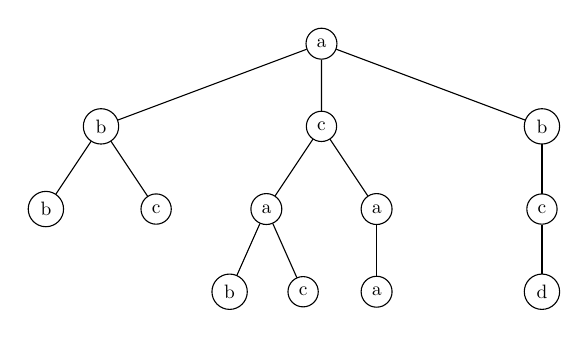
\begin{tikzpicture}[level/.style={sibling distance=40mm/#1}, scale=0.7,transform shape]
\node [circle,draw] (a) {a}
    child {node [circle,draw] (b) {b}
      child {node [circle, draw] {b}}
      child {node  [circle, draw] {c}}
    }
    child {node [circle,draw] (c) {c}
      child {node [circle,draw] (d) {a}
        child {node [circle, draw] {b}}
        child {node [circle, draw] {c}}
      }
      child {node [circle, draw] {a}
             child {node [circle,draw] (e) {a}
             }
            }
    }
    child {node [circle,draw] (b) {b}
      child {node  [circle, draw] {c}
        child {node [circle, draw] {d}}
            }
    }
;
\end{tikzpicture}
\end{center}
\caption{}
\end{subfigure}
%
%
\begin{subfigure}[b]{0.4\textwidth}
\begin{center}
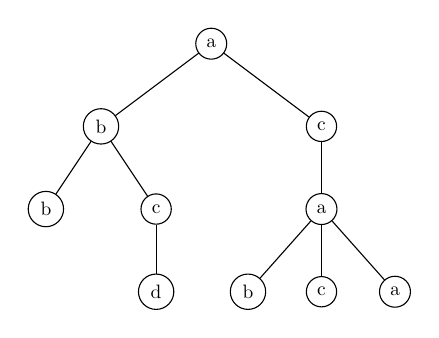
\begin{tikzpicture}[level/.style={sibling distance=40mm/#1}, scale=0.7,transform shape]
\node [circle,draw] (a) {a}
    child {node [circle,draw] (b) {b}
      child {node [circle, draw] {b}}
      child {node  [circle, draw] {c}
        child {node [circle, draw] {d}}
            }
    }
    child {node [circle,draw] (c) {c}
      child {node [circle, draw] {a}
        child {node [circle, draw] {b}}
        child {node [circle, draw] {c}}
             child {node [circle,draw] (e) {a}
             }
            }
    }
;
\end{tikzpicture}
\end{center}
\caption{}
\end{subfigure}
%
\caption{Illustration for Definition~\ref{def:psi}. Applying $\Psi$ to the tree in (a) results in the tree in (b). The trees have the same (not necessarily maximal) paths. In (b), no two siblings have the same label.}\label{fig:psi}% While $\La_1$ and $\La_2$ have disjoint images }
\end{figure}


\section{Decidability of 2-Distributivity}

We have shown that languages recognized by finite 2-distributive algebras form a subclass of PDL.
We now show that 2-distributivity is decidable.

%We defined $\pi(f)$ to be the set of paths in the forest $f$.
%If $\La$ is a language of forests, $\pi(\La) \subseteq Pow(\Sigma^*)$ is the image of $\La$ under $\pi$, a set of finite pathsets.
%Given a finite forest algebra $\Ff = (H,V)$, choose $\Sigma := V$, and let $\phi : \Sigma^\Delta \rightarrow (H,V)$ be the (unique) morphism extending the identity map $\phi : \Sigma \rightarrow V$, that is, mapping the context $v[X]$ to $v \in V$.
%We will see below that considering this morphism is sufficient when checking 2-distributivity.

To decide whether $\Ff$ is 2-distributive, we need to check for morphisms $\phi : \Sigma^\Delta\rightarrow\Ff$ whether $\phi(v(f_1+f_2)) = \phi(vf_1 + vf_2)$ holds whenever $\pi(f_1) = \pi(f_2)$, for all forests $f_1, f_2 \in H_\Sigma$ and all contexts $v \in V_\Sigma$.
To do this algorithmically, we want to find those pairs $h, h' \in H$ such that $\pi(\phi^{-1}(h))$ and $\pi(\phi^{-1}(h'))$ have nonempty intersection. For these $h, h'$, we then need to check whether $v(h+h') = vh+vh'$ for all $v \in V$. If we can find these pairs $h, h'$ algorithmically, decidability is shown (We will see that looking at one specific morphism $\phi$ is enough.).

Thus, the problem boils down to deciding, given two regular forest languages $\La_1, \La_2$, whether $\pi(\La_1) \cap \pi(\La_2)$ is empty.
We will reduce this to the problem of deciding whether two regular forest languages -- computed from $\La_1, \La_2$ -- have nonempty intersection.
We will use the following tool: %, which will also play a role in the proofs both of the Separation Lemma and the Local-Global Theorem:
\begin{defin}[Distributive Normal Form]\label{def:psi}
Define a map $\Psi : H_\Sigma \rightarrow H_\Sigma$ as follows.

Consider a forest $f := \beta_1[f_1] + ... + \beta_n[f_n]$ ($n \geq 0$).
Here, $\beta_1, ..., \beta_n$ are symbols from $\Sigma$, some or all of which can be identical, and $f_1, ..., f_n$ are forests.
For each $\beta \in \{\beta_1, .., \beta_n\}$, define \[F_\beta := \{f_i : \beta_i = \beta\} \subset \{f_1, ..., f_n\}\]
Then, set $$\Psi(f) := \sum_{\beta \in \{\beta_1, ..., \beta_n\}} \beta\left(\Psi\left[\sum_{f' \in F_\beta} f'\right]\right)$$


%Consider a tree $t := \alpha[\beta_1[t_1] + ... + \beta_n[t_n]]$.
%In order to compute $\Psi(\alpha[\beta_1[t_1] + ... + \beta_n[t_n]])$ ($\beta_i$ symbols from $\Sigma$, some or all of which can be identical), we can first collect the descendants $\{t^\beta_i\}$ from the set $\{t_1, ..., t_n\}$ for each symbol $\beta \in \{\beta_1, ...,  \beta_n\}$.
%Let $\beta^1, ..., \beta^k$ the unique elements of $\{\beta_1, ..., \beta_n\}$.
%Then, the result is $$\Psi(t) = \alpha\left[\sum_i \Psi\left(\beta^i\left[\sum_j t^{\beta_i}_j\right]\right)\right]$$
%
%
%Let's also write down a formal definition of $\Psi$.
%We can carry out the procedure starting at the root level and then go down until we reach the leaves.
%
%
%As long as the forest contains pairs of (distinct) siblings which the same root symbol, merge these to a single tree.
%This will reach a fixed point after finitely many steps.

%\emph{Should I add a formal definition?}
\end{defin}


%\begin{remark}
%Les formally, $\Psi(f)$ is obrained by iteratively merging 
%It is clear that, carrying this out recursively, we arrive at a forest where no two sibling nodes have the same symbol.
%\end{remark}
An example is provided in Figure~\ref{fig:psi}.

\begin{prop}\label{prop:psi}
Let $f, f' \in H_\Sigma$.
\begin{enumerate}
\item No two distinct sibling nodes in $\Psi(f)$ are labeled with the same symbol.

\item $\pi(f) = \pi(\Psi(f))$.

\item $\pi(f) = \pi(f')$ if and only if $\Psi(f) = \Psi(f')$.
\end{enumerate}
\end{prop}

\begin{proof}
(1) By induction over the height of forests.
(2) is immediate from the definition of $\Psi$.
For (3), the `if' direction follows from (2). For the `only if' direction, observe that, for any given pathset, there is only a single forest (up to order of siblings) having this pathset and satisfying the condition that no sibling nodes have the same symbol.
\end{proof}

Due to the second property, we will use $\Psi(f)$ as a suitable representative forest for the path set $\pi(f)$.
In certain ways, $\Psi(f)$ will be better-behaved than a general forest $f$.
The following proposition shows that the image of languages under $\Psi$ is also well-behaved:

\begin{prop}\label{prop:psi-reg}
Let $\La$ be a regular forest language. Then $\Psi(\La)$ is a regular forest language and can be effectively constructed from (an automaton for) $\La$.
\end{prop}

It is important to note that the image $\Psi(\La)$ is not recognized by a horizontally idempotent forest algebra, as multiplicity of children does matter. The recognizing finite forest algebra will be horizontally commutative but not idempotent.
This proposition and proof is the one place in this paper where we deviate from our convention that all forest algebras are horizontally commutative and idempotent.

\begin{proof}
%Recall the characterization of $\Psi$ from the Remark.
%Consider a nondeterministic top-down automaton for $\La$ with state set $Q$ and a set of rules $q_0 \leftarrow \alpha [q_1 + ... + q_k]$.
%We can construct a top-down automaton which, in state $\{q_1, ..., q_n\}$, selects a nonempty set of rules for each $q_i$, pools those rules together 

%From an automaton for $\La$ with state set $Q$, we can construct an automaton with state set $Pow(Q)$.


Let $\Ff = (H,V)$ be a finite forest algebra recognizing $\La$ via morphism $\phi$. 


Let $H' := {Pow(Pow(H))}^\Sigma \cup \{\bot\}$ with the operation: $f + f' = \bot$ if there is $\alpha \in \Sigma$ such that $f(\alpha), f'(\alpha) \neq \emptyset$, or if one of $f, f'$ is already equal to $\bot$.
Otherwise, $(f+f')(\alpha) = f(\alpha) \cup f'(\alpha)$.
It should be noted that this operation is not idempotent due to the first condition, which makes $f + f = \bot$ unless $f(\alpha) = \emptyset$ for all $\alpha$.
With this operation, $H'$ is a commutative finite monoid with identity $f_0$ given by $f_0(\alpha) = \emptyset$ for $\alpha \in \Sigma$.

Let $V'$ be the finite monoid of all maps $H' \rightarrow H'$, which naturally acts on $H'$.
It is easy to show that $(H',V')$ is a finite forest algebra (though not horizontally idempotent).

Then define a morphism $\psi : \Sigma^\Delta \rightarrow (H',V')$ by first constructing the images of the contexts consisting of only a single letter: $\psi(\alpha) := g_\alpha$ where by $\psi(\alpha)$ we denote the image of the context consisting of only $\alpha$ and a variable below it ($\alpha[X]$).
Once we have chosen $g_\alpha \in V'$ for each $\alpha$, it is not hard to see that we obtain a unique forest algebra morphism $\psi : \Sigma^\Delta \rightarrow (H',V')$ extending this map.
Recall that $g_\alpha$ will need to be a map $H' \rightarrow H'$.
We first set $g_\alpha(\bot) = \bot$ for all $\alpha$.
For $f \in H' - \{\bot\}$, so $f : \Sigma \rightarrow Pow(Pow(H))$, we furthermore set
\[\psi(\alpha)(f)(\beta) = \emptyset \text{ when }\alpha \neq \beta\]
Finally, considering the case $\alpha = \beta$, then for any $Q \subset H$, we set $Q \in \psi(\alpha)(f)(\alpha)$ if and only if
there are sets $Q_1, ..., Q_l \subset H$ such that for each $\gamma \in \Sigma$ such that $f(\gamma) \neq \emptyset$, there is $P_\gamma \in f(\gamma)$ such that
\[Q_1 \cup ... \cup Q_l = \bigcup_{\gamma} P_\gamma\]
 and 
\[Q = \left\{\phi(\alpha)\cdot\left[\sum_{h \in Q_i} h\right] : i=1, ..., l\right\}\]
%First, it is clear that $\psi(f) = \bot$ if and only if two sibling nodes within $f$ have the same symbol.
%
%For any tree $t$ in the image of $\Psi$ (that is, no two sibling nodes have the same symbol).
%
%We now claim that, for a forest $f = \{t_{\alpha_k} : i = 1, ..., k\}$, where the tree $t_i^{\alpha_j}$ has $\alpha_j$ as the symbol of its root node,
%we have $$\psi(f) = \{f : f(\alpha)
%
We now claim that, for $h \in H$, the language $\Psi(\phi^{-1}(h)) - \{\emptyset\}$ (that is, removing the empty forest if it is in the language) is equal to 
\[\psi^{-1}(\{f : \exists \alpha : f(\alpha) \neq \emptyset \wedge \forall \alpha \in \Sigma : f(\alpha) = \emptyset \vee \{h\} \in f(\alpha)\})\]
where $\psi$ is the forest algebra morphism $\psi : \Sigma^\Delta \rightarrow (H',V')$ that we just constructed.
This is shown by induction over forests.

Considering that the empty forest is the only element of the preimage of the identity element of $H'$, this implies that $\Psi(\La)$ is recognized by $(H',V')$ via $\psi$.
\end{proof}



We can now show decidability of 2-distributivity:
\begin{theorem}\label{prop:2-decid}
It is decidable whether a finite forest algebra is 2-distributive.
\end{theorem}

\begin{proof}
Given a finite forest algebra $\Ff = (H,V)$, choose $\Sigma := V$, and let $\phi : \Sigma^\Delta \rightarrow (H,V)$ be the (unique) morphism extending the identity map $\phi : \Sigma \rightarrow V$, that is, mapping the context $v[X]$ to $v \in V$.

Given two regular forest languages $\La_1, \La_2$, it is decidable whether $\pi(\La_1) \cap \pi(\La_2)$ is empty.
To prove this, we use the mapping $\Psi$ introduced in Definition~\ref{def:psi}.
We can use Proposition~\ref{prop:psi-reg} to effectively check whether the regular forest languages $\Psi(\La_1)$ and $\Psi(\La_2)$ have nonempty intersection.
From Proposition~\ref{prop:psi}, we know that this happens if and only if $\pi(\phi^{-1}(h))$ and $\pi(\phi^{-1}(h'))$ also have nonempty intersection.

Using this resut, we can then, for each pair $h, h' \in H$, effectively check whether $\pi(\phi^{-1}(h))$ and $\pi(\phi^{-1}(h'))$ have nonempty intersection.
If this is the case, we can check for each context type $v \in V$ whether $v[h+h'] = vh+vh'$.
This equality holds for each $v$ and for each selected pair $h, h'$ if and only if $\phi(c(f+f')) = \phi(cf+cf')$ for all $c \in V_\Sigma$ and each $f, f' \in H_\Sigma$ such that $\pi(f) = \pi(f')$.
This is a necessary condition for $\Ff$ to be 2-distributive.


To prove that this is also sufficient, consider another alphabet $\Sigma'$ and a morphism $\psi : \Sigma'^\Delta \rightarrow (H,V)$.
We can build a morphism $\eta : \Sigma'^\Delta \rightarrow \Sigma^\Delta$, generated by the map $\Sigma' \rightarrow \Sigma$ defined by $\eta(\alpha) := \psi(\alpha) \in \Sigma$ for $\alpha \in \Sigma'$.
Then $\psi = \phi \circ \eta$.
Let $f_1, f_2 \in H_{\Sigma'}$ with $\pi(f_1) = \pi(f_2)$, and let $c \in V_{\Sigma'}$.
Then $\pi(\eta(f_1)) = \pi(\eta(f_2))$, and, by assumption, $\psi(c[f_1+f_2]) = \phi(\eta(c[f_1+f_2])) = \phi(\eta(c)[\eta(f_1)+\eta(f_2)]) = \phi(\eta(c)\eta(f_1)+\eta(c)\eta(f_2)) = \phi(\eta(cf_1+cf_2)) = \psi(cf_1+cf_2)$.





%Appendix~\ref{sec:proof-2-decid}.
\end{proof}





\section{Discussion}\label{sec:discussion}

We have shown that 2-distributive finite forest algebras recognize a subclass of PDL, and that 2-distributivity is a decidable property.

As we outlined in the Introduction, generalizing this approach to $k > 2$ would settle decidability of PDL.
Our notion of 2-distributivity can be generalized in the following way, slightly different than the one given in~\cite{straubing-new-2013}:


\begin{defin}
For each $k \geq 1$, define a congruence $\sim_k$ on $\Sigma^\Delta = (H_\Sigma, V_\Sigma)$ as follows:
\begin{enumerate}
\item $\sim_1$ is the smallest congruence such that $f \sim_1 f'$ whenever $f, f' \in H_\Sigma$ and $\pi(f) = \pi(f')$.
\item For any $k \geq 1$, $\sim_{k+1}$ is the smallest congruence such that \[v[f+f'] \sim_{k+1} vf + vf'\] for any $v \in V_\Sigma$ and any $f, f' \in H_\Sigma$ such that $f \sim_k f'$.
\end{enumerate}
\end{defin}
For each $k$, the congruence $\sim_k$ encodes a $k$-fold iteration of the distributive law.
A forest algebra $\Ff$ is \emph{$k$-distributive} if, for all morphisms $\phi : \Sigma^\Delta \rightarrow \Ff$, $\phi(f) = \phi(f')$ whenever $f \sim_k f'$.
For $k = 2$, this coincides with our definition above.

In analogy to Proposition~\ref{prop:wreath-2} and a result from ~\cite{straubing-new-2013}, it can be shown that the wreath product of $k$ distributive forest algebras is k-distributive.
Determining, given a finite forest algebra $\Ff$, whether it is $k$-distributive for some $k$ is a decidable problem.
If one could show that any finite $k$-distributive forest algebra only recognizes languages in PDL, definability in PDL would therefore be shown decidable~\cite{straubing-new-2013}.
We have solved this problem in the case $k=2$.

Indeed, generalizing our Local-Global Theorem to $k \geq 2$ is feasible, and the proof method of our main result might be adapted to construct an inductive proof.
It would be sufficient to, given a general $k$-distributive algebra, construct a wreath product of finite distributive algebras and show that an appropriate derived forest algebra is $k-1$-distributive. 
To carry this out, a suitable strengthening of our Separation Lemma to a property stronger than separation would be required.


PDL is a member of a larger family of forest languages for which decidability of expressibility is still unknown, in spite of longstanding interest and several attempts \cite{thomas-logical-1984,  potthoff-first-order-1995}. %\cite{thomas-chain-1987},
For a range of tree and forest logics, decidable characterizations have been obtained (see \cite{bojanczyk-effective-2008} for a survey up to 2008; more recent results include \cite{bojanczyk-piecewise-2012,bojanczyk-tree-2010,place-deciding-2010,place-decidable-2009,benedikt-regular-2009} among others).
However, for many more prominent logics, including First-Order Logic with ancestor, $CTL$, $CTL^*$, PDL, and Chain Logic, this problem remains open.
As described in the introduction, PDL extends both $CTL$ and $CTL^*$.
All of these logics were shown by \cite{bojanczyk-wreath-2012} to correspond to iterated wreath products of specific types of forest algebras satisfying a distributive law.
Among these, PDL stands out because it is characterized through products of arbitrary distributive forest algebras, and can -- at least at the level $k = 2$ -- be captured in terms of a $k$-fold iterated distributive law.
Therefore, our results might also shed light on this larger family of open problems.



In the field of regular word languages and logic on words, the study of finite monoids has been tremendously successful.
Our proof strategy highlights how the classical theory developed for studying logic on words via wreath products of monoids carries over faithfully to the setting of forest algebras:
Our proof proceeds by solving two sub-problems related to the left and right factors in wreath product decompositions: a separation result and a Local-Global theorem, which are then combined via the Derived Category Theorem \cite{tilson-categories-1987}.
These steps are remarkably similar to results from the theory of logic on words and finite monoids which also reduce the problem of decidability to separation \cite{place-going-2014} and Local-Global theorems \cite{krebs-effective-2012}.



%\bibliographystyle{apalike}
\bibliography{references}
\end{document}

